% Options for packages loaded elsewhere
\PassOptionsToPackage{unicode}{hyperref}
\PassOptionsToPackage{hyphens}{url}
%
\documentclass[
]{book}
\usepackage{amsmath,amssymb}
\usepackage{lmodern}
\usepackage{iftex}
\ifPDFTeX
  \usepackage[T1]{fontenc}
  \usepackage[utf8]{inputenc}
  \usepackage{textcomp} % provide euro and other symbols
\else % if luatex or xetex
  \usepackage{unicode-math}
  \defaultfontfeatures{Scale=MatchLowercase}
  \defaultfontfeatures[\rmfamily]{Ligatures=TeX,Scale=1}
\fi
% Use upquote if available, for straight quotes in verbatim environments
\IfFileExists{upquote.sty}{\usepackage{upquote}}{}
\IfFileExists{microtype.sty}{% use microtype if available
  \usepackage[]{microtype}
  \UseMicrotypeSet[protrusion]{basicmath} % disable protrusion for tt fonts
}{}
\makeatletter
\@ifundefined{KOMAClassName}{% if non-KOMA class
  \IfFileExists{parskip.sty}{%
    \usepackage{parskip}
  }{% else
    \setlength{\parindent}{0pt}
    \setlength{\parskip}{6pt plus 2pt minus 1pt}}
}{% if KOMA class
  \KOMAoptions{parskip=half}}
\makeatother
\usepackage{xcolor}
\IfFileExists{xurl.sty}{\usepackage{xurl}}{} % add URL line breaks if available
\IfFileExists{bookmark.sty}{\usepackage{bookmark}}{\usepackage{hyperref}}
\hypersetup{
  pdftitle={Python - Guia do Programador},
  pdfauthor={Peter Jandl Junior},
  hidelinks,
  pdfcreator={LaTeX via pandoc}}
\urlstyle{same} % disable monospaced font for URLs
\usepackage{color}
\usepackage{fancyvrb}
\newcommand{\VerbBar}{|}
\newcommand{\VERB}{\Verb[commandchars=\\\{\}]}
\DefineVerbatimEnvironment{Highlighting}{Verbatim}{commandchars=\\\{\}}
% Add ',fontsize=\small' for more characters per line
\usepackage{framed}
\definecolor{shadecolor}{RGB}{248,248,248}
\newenvironment{Shaded}{\begin{snugshade}}{\end{snugshade}}
\newcommand{\AlertTok}[1]{\textcolor[rgb]{0.94,0.16,0.16}{#1}}
\newcommand{\AnnotationTok}[1]{\textcolor[rgb]{0.56,0.35,0.01}{\textbf{\textit{#1}}}}
\newcommand{\AttributeTok}[1]{\textcolor[rgb]{0.77,0.63,0.00}{#1}}
\newcommand{\BaseNTok}[1]{\textcolor[rgb]{0.00,0.00,0.81}{#1}}
\newcommand{\BuiltInTok}[1]{#1}
\newcommand{\CharTok}[1]{\textcolor[rgb]{0.31,0.60,0.02}{#1}}
\newcommand{\CommentTok}[1]{\textcolor[rgb]{0.56,0.35,0.01}{\textit{#1}}}
\newcommand{\CommentVarTok}[1]{\textcolor[rgb]{0.56,0.35,0.01}{\textbf{\textit{#1}}}}
\newcommand{\ConstantTok}[1]{\textcolor[rgb]{0.00,0.00,0.00}{#1}}
\newcommand{\ControlFlowTok}[1]{\textcolor[rgb]{0.13,0.29,0.53}{\textbf{#1}}}
\newcommand{\DataTypeTok}[1]{\textcolor[rgb]{0.13,0.29,0.53}{#1}}
\newcommand{\DecValTok}[1]{\textcolor[rgb]{0.00,0.00,0.81}{#1}}
\newcommand{\DocumentationTok}[1]{\textcolor[rgb]{0.56,0.35,0.01}{\textbf{\textit{#1}}}}
\newcommand{\ErrorTok}[1]{\textcolor[rgb]{0.64,0.00,0.00}{\textbf{#1}}}
\newcommand{\ExtensionTok}[1]{#1}
\newcommand{\FloatTok}[1]{\textcolor[rgb]{0.00,0.00,0.81}{#1}}
\newcommand{\FunctionTok}[1]{\textcolor[rgb]{0.00,0.00,0.00}{#1}}
\newcommand{\ImportTok}[1]{#1}
\newcommand{\InformationTok}[1]{\textcolor[rgb]{0.56,0.35,0.01}{\textbf{\textit{#1}}}}
\newcommand{\KeywordTok}[1]{\textcolor[rgb]{0.13,0.29,0.53}{\textbf{#1}}}
\newcommand{\NormalTok}[1]{#1}
\newcommand{\OperatorTok}[1]{\textcolor[rgb]{0.81,0.36,0.00}{\textbf{#1}}}
\newcommand{\OtherTok}[1]{\textcolor[rgb]{0.56,0.35,0.01}{#1}}
\newcommand{\PreprocessorTok}[1]{\textcolor[rgb]{0.56,0.35,0.01}{\textit{#1}}}
\newcommand{\RegionMarkerTok}[1]{#1}
\newcommand{\SpecialCharTok}[1]{\textcolor[rgb]{0.00,0.00,0.00}{#1}}
\newcommand{\SpecialStringTok}[1]{\textcolor[rgb]{0.31,0.60,0.02}{#1}}
\newcommand{\StringTok}[1]{\textcolor[rgb]{0.31,0.60,0.02}{#1}}
\newcommand{\VariableTok}[1]{\textcolor[rgb]{0.00,0.00,0.00}{#1}}
\newcommand{\VerbatimStringTok}[1]{\textcolor[rgb]{0.31,0.60,0.02}{#1}}
\newcommand{\WarningTok}[1]{\textcolor[rgb]{0.56,0.35,0.01}{\textbf{\textit{#1}}}}
\usepackage{longtable,booktabs,array}
\usepackage{calc} % for calculating minipage widths
% Correct order of tables after \paragraph or \subparagraph
\usepackage{etoolbox}
\makeatletter
\patchcmd\longtable{\par}{\if@noskipsec\mbox{}\fi\par}{}{}
\makeatother
% Allow footnotes in longtable head/foot
\IfFileExists{footnotehyper.sty}{\usepackage{footnotehyper}}{\usepackage{footnote}}
\makesavenoteenv{longtable}
\usepackage{graphicx}
\makeatletter
\def\maxwidth{\ifdim\Gin@nat@width>\linewidth\linewidth\else\Gin@nat@width\fi}
\def\maxheight{\ifdim\Gin@nat@height>\textheight\textheight\else\Gin@nat@height\fi}
\makeatother
% Scale images if necessary, so that they will not overflow the page
% margins by default, and it is still possible to overwrite the defaults
% using explicit options in \includegraphics[width, height, ...]{}
\setkeys{Gin}{width=\maxwidth,height=\maxheight,keepaspectratio}
% Set default figure placement to htbp
\makeatletter
\def\fps@figure{htbp}
\makeatother
\setlength{\emergencystretch}{3em} % prevent overfull lines
\providecommand{\tightlist}{%
  \setlength{\itemsep}{0pt}\setlength{\parskip}{0pt}}
\setcounter{secnumdepth}{5}
\usepackage{booktabs}
\usepackage{amsthm}
\makeatletter
\def\thm@space@setup{%
  \thm@preskip=8pt plus 2pt minus 4pt
  \thm@postskip=\thm@preskip
}
\makeatother
\ifLuaTeX
  \usepackage{selnolig}  % disable illegal ligatures
\fi
\usepackage[]{natbib}
\bibliographystyle{apalike}

\title{Python - Guia do Programador}
\author{Peter Jandl Junior}
\date{2021-06-28}

\begin{document}
\maketitle

{
\setcounter{tocdepth}{1}
\tableofcontents
}
\hypertarget{prefuxe1cio}{%
\chapter*{Prefácio}\label{prefuxe1cio}}
\addcontentsline{toc}{chapter}{Prefácio}

Este é um livro experimental, organizado com o propósito de incentivar o uso da linguagem de programação Python e, sendo assim, procura cobrir os aspectos mais básicos de sua utilização, bem como alguns conceitos fundamentais e boas práticas da programação. Para tanto, apresenta os elementos básicos da linguagem, ao mesmo tempo que trata dos aspectos básicos da programação, prosseguindo para conceitos e técnicas mais avançados.

Será utilizada a versão 3 do Python, que é substancialmente diferente da versão 2 e, também, considerada mais correta semanticamente falando, além de suportar um conjunto de novas e interessantes características.

Este material foi escrito com \textbf{R Markdown} e uso do pacote \textbf{bookdown}\footnote{Bookdown no GitHub: \url{https://github.com/rstudio/bookdown}.} \citep{R-bookdown, xie2015}, portanto emprega o suporte do \textbf{Pandoc}, como, por exemplo, para indicar expressões matemáticas, tal como \(f(x) = a*x^2 + b*x + c\).

O muitos fragmentos de código e exemplos contidos neste material aparecem como segue. Quando incluída, a saída produzida pelos fragmentos aparecerá imediatamente a seguir do código apresentado, precedida pelos caracteres \texttt{\textgreater{}\textgreater{}\textgreater{}}.

\begin{Shaded}
\begin{Highlighting}[]
\CommentTok{\# Uma mensagem de boas vindas}
\BuiltInTok{print}\NormalTok{(}\StringTok{\textquotesingle{}Bem vindo ao "Python {-} Guia do Programador"!\textquotesingle{}}\NormalTok{)}
\end{Highlighting}
\end{Shaded}

\begin{verbatim}
>>> Bem vindo ao "Python - Guia do Programador"!
\end{verbatim}

Este material será futuramente armazenado no \textbf{GitHub}, no repositório: \url{https://github.com/pjandl/pygp}.

\hypertarget{intro}{%
\chapter{Introdução}\label{intro}}

\textbf{Python} é uma linguagem de programação bastante popular, moderna, utilizada tanto no ambiente corporativo, como no meio acadêmico, e que todo programador devia conhecer. Segundo Kopec \citep[pág.1]{kop2019}:

\begin{quote}
``Python é usada em atividades tão diversas como ciência de dados, produção de filmes, educação em ciência da computação, gerenciamento de tecnologia da informação e muito mais. Realmente não há um ramo da computação que Python não tenha tocado (exceto, talvez, desenvolvimento de \emph{kernel} de sistemas operacionais). Python é amada por sua flexibilidade, sintaxa bela e suscinta, orientação a objetos pura, e uma comunidade movimentada.''
\end{quote}

Então, vamos falar um pouco sobre ela!

\hypertarget{introd-histo}{%
\section{Breve Histórico}\label{introd-histo}}

Observando as dificuldades de muitas pessoas em aprender a programar e trabalhar com programação, Guido Van Rossun, que então trabalhava no \href{http://www.cwi.nl/}{\emph{Stichting Mathematish Centrum}} (CWI, Holanda), deu início ao desenvolvimento de uma nova linguagem de programação em 1990. Sua proposta era oferecer um linguagem de \emph{script} simples, fácil de aprender e de programar. O nome \textbf{Python} foi inspirado pelo grupo humorístico britânico \emph{Monty Python}, criador do programa de televisão \emph{Monty Python's Flying Circus}.

Em 1995, já no \emph{Corporation for National Research Initiatives} (EUA), Rossun, deu continuidade ao seu projeto de tornar o Python ainda melhor, neste ponto com as opiniões e ajuda de várias outras pessoas contribuíram no desenvolvimento da linguagem e de suas bibliotecas.

Para garantir a evolução contínua da linguagem e, ao mesmo tempo, desvincular o Python da pessoa de Guido Van Rossun, foi criada em 2001 a \href{https://www.python.org/psf/}{\emph{Python Software Foundation}} (PSF), uma organização sem fins lucrativos, que detém os direitos de propriedade intelectual do Python, destinada a manter, desenvolver e divulgar a linguagem com base em um modelo de desenvolvimento comunitário, aberto, com participação de membros individuais e corporativos.

Todas as versões do Python são de \emph{código aberto}\footnote{Veja uma definição de \emph{código aberto} ou \emph{open source} em \url{http://www.opensource.org/}.}.

\hypertarget{introd-carac}{%
\section{Características}\label{introd-carac}}

Python é uma linguagem de programação de alto nível, orientada a objetos, interpretada, interativa, de semântica dinâmica, com tipagem forte. Sua sintaxe é bastante compacta e direta, o que possibilita aos seus programas serem mais curtos do que os construídos em C, C++, Java e outras linguagens.

As razões para isso são:

\begin{itemize}
\tightlist
\item
  dispõe de tipos de dados de alto nível que permitem a expressão direta de operações complexas;
\item
  não requer a declaração prévia de variáveis ou argumentos, cujos tipos são inferidos durante a execução do programa;
\item
  a criação de blocos de diretivas nas suas construções requer apenas a indentação simples, sem necessidade de elementos extras, como chaves ou palavras reservadas, para identificação de início e fim de tais blocos.
\end{itemize}

Foi projetada para ser simples e elegante, ao mesmo que é sofisticada e completa, pois:

\begin{itemize}
\tightlist
\item
  é orientada a objetos, oferece herança simples, herança múltipla e tratamento polimórfico de objetos;
\item
  oferece exceções como mecanismo mais moderno para o tratamento de erros;
\item
  possui coleta automática de lixo, que efetua a reciclagem de memória de objetos descartados, simplificando o desenvolvimento;
\item
  inclui recursos avançados de manipulação de texto, listas e outras estruturas de dados; e
\item
  seus programas podem ser organizados em módulos e pacotes, reusáveis em diferentes programas.
\end{itemize}

Pode ser usada em múltiplas plataformas (Mac OS, Microsoft Windows, distribuições Linux e Unix), o que evidencia sua portabilidade\footnote{\emph{Portabilidade} é a capacidade dos programas gerados por uma linguagem de programação de serem executados em diferentes plataformas operacionais, idealmente sem alterações, ou com um mínimo de modificações.}. Além de ser extensível e dotada de uma ampla e versátil biblioteca.

Como característica de seu projeto, a linguagem Python possui um interpretador que pode funcionar em modo interativo. Isto possibilita que programas escritos em Python, ou mesmo trechos de código, possam ser testados antes de serem compilados ou inclusos em outros programas. Com isso, o Python encoraja a programação de maneira simples, sem requisitar código burocrático, o que a torna muito conveniente para criação rápida de programas.

Por tudo isso é muito utilizada para tratamento, processamento de visualização de dados em aplicações de Análise de Dados (\emph{Data Analysis}) e de Ciência de Dados (\emph{Data Science}). Mas tambem é empregada na construção de aplicações complexas e de grande porte em empresas icônicas como DropBox, Google, IBM, Instagram, Nasa, Reddit, Spotify, Uber, YouTube e outras.

\hypertarget{introd-habil}{%
\section{Habilidades da Programação}\label{introd-habil}}

\emph{Programar}\footnote{Dicio (Dicionário On-Line de Português): \url{https://www.dicio.com.br/programar/}.} significa \emph{fazer o programa de, planejar, incluir em programação}, além de ter como sinônimos \emph{planejar, projetar, delinear, designar e coordenar}.

A programação de computadores exige o domínio de seis habilidades distintas:

\begin{enumerate}
\def\labelenumi{\arabic{enumi}.}
\tightlist
\item
  computação (Capítulo \ref{comput}),
\item
  entrada e saída (Capítulo \ref{e-s}),
\item
  repetição (Capítulo \ref{repet}),
\item
  decisão (Capítulo \ref{decis}),
\item
  modularização (Capítulo \ref{modul}), e
\item
  sequenciação (Capítulo \ref{seque}).
\end{enumerate}

A \emph{computação} é habilidade necessária para expressar e realizar cálculos, ou seja, a capacidade de combinar valores, variáveis, operadores e funções para obter os resultados desejados. Esta habilidade explora as capacidades dos computadores em realizar cálculos.

Os dados necessários para realizar os cálculos desejados, isto é, requeridos pela computação, precisam ser obtidos dos usuários ou outras fontes de dados. Da mesma maneira, os resultados produzidos por um programa precisam ser exibidos para seus usuários. Estas são as operações de \emph{entrada e saída}, simples mas essenciais.

A \emph{repetição} consiste da identificação de uma instrução ou um conjunto de instruções que devem ser executados mais de uma vez, o que inclui determinar o número de vezes que tais instruções serão executadas ou a condição que exige sua repetição. Além disso, a repetição permite reduzir a quantidade de instruções necessárias para resolver um problema, e confere maior flexibilidade às soluções criadas.

Outra habilidade importante é a \emph{decisão}, pois possibilita escolher quais instruções serão executadas, isto é, permite que, durante a execução das instruções, sejam selecionadas aquelas que serão executadas. Esta decisão é realizada mediante a avaliação de uma condição que o programador estabelece como critério de escolha ou de seleção.

A \emph{modularização}, que é a habilidade que trata da divisão das instruções necessárias para resolução de um problema em partes menores, cada uma com responsabilidades distintas. Essa estratégia oferece várias vantagens, entre elas, simplificar a compreensão e solução do problema, além de possibilitar o reuso.

Finalmente temos a \emph{sequenciação}, que se refere a habilidade de organizar as instruções de um programa de maneira tal que seja resolvido um problema específico. Esta habilidade trata de estabelecer uma sequência adequada de instruções para solução de um problema, ou seja, ela representa a \emph{lógica} com a qual resolvemos um problema. A sequenciação determina como os dados de um problema serão processados, portanto combina todas as habilidades anteriores: a entrada e saída, a computação, a repetição, a decisão e a modularização necessárias para a construção de um programa.

\hypertarget{comput}{%
\chapter{Computação}\label{comput}}

A palavra \emph{computar}\footnote{Dicio (Dicionário On-Line de Português): \url{https://www.dicio.com.br/computar}.} significa \emph{fazer o cômputo de, calcular, orçar}, assim, a \emph{computação} é a habilidade da programação voltada para a realização de cálculos, o que permite explorar uma das capacidades centrais dos computadores.

A realização de cálculos envolve a construção de \emph{expressões}, as quais podem conter vários elementos:

\begin{itemize}
\tightlist
\item
  valores literais,
\item
  variáveis,
\item
  operadores, e
\item
  funções.
\end{itemize}

\hypertarget{comput-liter}{%
\section{Valores Literais}\label{comput-liter}}

Um \emph{valor literal}, ou apenas \emph{literal}, é uma quantidade, um número, uma palavra, um nome ou um texto que podemos ler diretamente numa instrução, isto é, um elemento que não depende da execução da instrução ou de qualquer outra parte do programa para que possa ser compreendido. Alguns exemplos podem facilitar no entendimento do que são os literais.

O número \texttt{2021} é um literal, assim como \texttt{15}, \texttt{3.14}, \texttt{-3} ou \texttt{4294967296} também são literais numéricos, que são escritos diretamente no texto do programa Python, tal como em todas as linguagens de programação. Vale notar que o \emph{separador} decimal é o caractere ponto (\texttt{.}).

Já a inclusão de literais de texto no Python, seja uma palavra, frase ou um caractere individual, requer que sejam dispostos entre aspas simples (\texttt{\textquotesingle{}}) ou aspas duplas (\texttt{"}). Estes \emph{delimitadores} de texto podem ser usados para indicar palavras, como \texttt{\textquotesingle{}computador\textquotesingle{}} ou \texttt{"programação"}, e caracteres individuais, como \texttt{\textquotesingle{}A\textquotesingle{}}, \texttt{"x"}, \texttt{\textquotesingle{}!\textquotesingle{}}, \texttt{"@"} ou \texttt{\textquotesingle{}+\textquotesingle{}}. Pequenas frases, que não podem exceder uma linha, são indicadas da mesma maneira, ou seja, com uso destes delimitadores, como no fragmento que segue.

\begin{Shaded}
\begin{Highlighting}[]
\CommentTok{\textquotesingle{}Python é uma linguagem de programação moderna.\textquotesingle{}}
\CommentTok{"A área de \textquotesingle{}data science\textquotesingle{} utiliza Python."}
\CommentTok{\textquotesingle{}A linguagem Python é "interpretada" e "dinâmica".\textquotesingle{}}
\end{Highlighting}
\end{Shaded}

Os delimitadores são exigidos para que seja possível distinguir o texto literal fornecidos pelo programador dos demais elementos da linguagem. O delimitador não pode fazer parte do texto delimitado, no entanto, é interessante observar que as aspas simples podem usadas quando delimitadas por aspas duplas e vice-versa.

Também é possível definir texto literal com múltiplas linhas, com o uso triplo de aspas simples ou aspas duplas, o que pode ser conveniente em algumas situações, como por exemplo indicar comandos SQL\footnote{\emph{Structured Query Language}, linguagem padronizada para consulta e manipulação de dados em \emph{Sistemas Gerenciadores de Bancos de Dados Relacionais} (SGBDR).} usados pelo programa. Seguem exemplos diretos.

\begin{Shaded}
\begin{Highlighting}[]
\CommentTok{"""Python is used in pursuits as diverse as data science,}
\CommentTok{film{-}making, computer science education, IT management, }
\CommentTok{and much more."""}

\CommentTok{\textquotesingle{}\textquotesingle{}\textquotesingle{}There really is no computing field that Python has not }
\CommentTok{touched (except maybe kernel development). Python is loved}
\CommentTok{for its flexibility, beautiful and succinct syntax, }
\CommentTok{object{-}oriented purity, and bustling community.}

\CommentTok{{-}{-}{-} Kopec (2019)\textquotesingle{}\textquotesingle{}\textquotesingle{}}
\end{Highlighting}
\end{Shaded}

Além de literais numéricos e de texto, o Python também dispõe de dois literais de tipo lógico (ou boleanos), que são \texttt{False} e \texttt{True}, que respectivamente representam os estados \emph{falso} e \emph{verdadeiro}.

\hypertarget{comput-tipos}{%
\section{Tipos de Dados}\label{comput-tipos}}

A linguagem Python é capaz de lidar com vários tipos de dados, ou seja, com categorias distintas de valores, cada uma oferecendo um conjunto próprio de possibilidades. Os tipos de dados básicos disponíveis na linguagem são considerados tipos \emph{built-in}\footnote{O termo \emph{built-in} é utilizado para designar um elemento que faz parte da própria definição da linguagem, ou seja, está disponível em todos os programas, sem necessidade de importação de módulos ou pacotes.}, ou \emph{nativos}, e estão listados na Tabela 2.1.

Tabela 2.1: Tipos de dados \emph{built-in}

\begin{longtable}[]{@{}
  >{\raggedright\arraybackslash}p{(\columnwidth - 2\tabcolsep) * \real{0.14}}
  >{\raggedright\arraybackslash}p{(\columnwidth - 2\tabcolsep) * \real{0.86}}@{}}
\toprule
Tipo & Descrição \\
\midrule
\endhead
\texttt{int} & Inteiro (ou integral), valor númerico sem parte fracionária. \\
\texttt{float} & Real, valor numérico com parte fracionária em ponto flutuante. \\
\texttt{bool} & Lógico (ou boleano). \\
\texttt{string} & \emph{String} ou cadeia de caracteres. \\
\texttt{complex} & Número complexo, com a parte imaginária identificada pelo sufixo \texttt{j}. \\
\bottomrule
\end{longtable}

O Python dispõe de três tipos de dados numéricos \emph{built-in}: \texttt{int}, \texttt{float} e \texttt{complex}. O tipo \texttt{int} possibilita a representação de valores numéricos inteiros, ou seja, números, contagens e quantidades, positivos ou negativos, mas sem uma parte fracionária. A função \emph{built-in} \texttt{type()} permite determinar o tipo de quaisquer valores literais (na verdade, de qualquer coisa no Python). Observe o uso de \texttt{type()} para o valor inteiro \texttt{15}.

\begin{Shaded}
\begin{Highlighting}[]
\BuiltInTok{type}\NormalTok{(}\DecValTok{15}\NormalTok{)}
\end{Highlighting}
\end{Shaded}

\begin{verbatim}
>>> <class 'int'>
\end{verbatim}

Qualquer valor inteiro, quando avaliado por \texttt{type()}, produz como retorno a classe \texttt{int}, que representa este tipo de dados.

Analogamente, o tipo \texttt{float} possibilita a representação de valores numéricos reais, ou seja, números positivos ou negativos dotados de uma parte fracionária. Como antes, pode ser usada a função \emph{built-in} \texttt{type()} para determinar o tipo de literais reais, como segue.

\begin{Shaded}
\begin{Highlighting}[]
\BuiltInTok{type}\NormalTok{(}\FloatTok{3.14}\NormalTok{)}
\end{Highlighting}
\end{Shaded}

\begin{verbatim}
>>> <class 'float'>
\end{verbatim}

Valores reais avaliados por \texttt{type()} produzem como retorno a classe \texttt{float}, que representa este tipo de dados.

Diferente da grande maioria das linguagens de programação, Python permite a representação nativa de números complexos, ou seja, valores dotados de uma parte real e uma parte imaginária, que utiliza o sufixo \texttt{j} para diferenciá-la da parte real. No fragmento que segue, a função \texttt{type()} é utilizada para determinar o tipo do valor literal \texttt{1.5\ -\ 4.9j}, um número complexo cuja parte real tem valor \texttt{1.5} e a parte imaginária vale \texttt{4.9j}.

\begin{Shaded}
\begin{Highlighting}[]
\BuiltInTok{type}\NormalTok{(}\FloatTok{1.5} \OperatorTok{{-}} \OtherTok{4.9j}\NormalTok{)}
\end{Highlighting}
\end{Shaded}

\begin{verbatim}
>>> <class 'complex'>
\end{verbatim}

A verificação de tipo com \texttt{type()} retorna a classe \texttt{complex} quando recebe números complexos como argumento.

Outro importante tipo \emph{built-in} é \texttt{bool} que representa o tipo lógico ou boleano, que possui apenas dois valores possíveis: \texttt{False}, para valores falsos; e \texttt{True}, para valores verdadeiros. O uso de \texttt{type()} para o literal lógico \texttt{True} é mostrado no fragmento que segue.

\begin{Shaded}
\begin{Highlighting}[]
\BuiltInTok{type}\NormalTok{(}\VariableTok{True}\NormalTok{)}
\end{Highlighting}
\end{Shaded}

\begin{verbatim}
>>> <class 'bool'>
\end{verbatim}

Como esperado, é retornada a classe \texttt{bool}.

Finalmente, a representação de texto, sejam caracteres, palavras ou frases, é feita por \emph{strings}, ou seja, elementos do tipo \texttt{str}, à despeito do delimitador usado (aspas simples, duplas ou triplas). A função \texttt{type()} também permite determinar o tipo de literais ou valores de texto, como segue.

\begin{Shaded}
\begin{Highlighting}[]
\BuiltInTok{type}\NormalTok{(}\StringTok{\textquotesingle{}Python: Guia do programador\textquotesingle{}}\NormalTok{)}
\end{Highlighting}
\end{Shaded}

\begin{verbatim}
>>> <class 'str'>
\end{verbatim}

Observamos que a classe \texttt{str} é retornada quando \texttt{type()} verifica o tipo de uma \emph{string}, ou seja, quando se fornece um argumento de texto.

\hypertarget{comput-varia}{%
\section{Variáveis}\label{comput-varia}}

Um programa de computador requer o uso de alguns ou de muitos dados para que possa produzir os resultados desejados. Durante a execução do programa, os dados necessários são armazenados na memória do computador. Para evitar que o programador tenha que lidar com os endereços de memória, isto é, com as posições onde os dados ficam efetivamente armazenados, são utilizadas \emph{variáveis}.

Uma \emph{variável} é um espaço em memória, reservado para guardar um valor, ao qual se associa um \emph{identificador}, ou seja, um nome por meio do qual se define e se recupera o valor armazenado. O uso de variáveis simplifica a programação, pois o programador não precisa se preocupar com os endereços de memória utilizados, nem com o espaço necessário (número de bytes) para armazenar tais valores, tão pouco com a organização dos dados e das instruções do programa.

Por meio do uso das variáveis, o programador pode armazenar valores literais ou o resultado de cálculos diversos, que podem ser utilizados em etapas posteriores do programa, evitando sua repetição e o processamento destes cálculos.

Além disso, o uso de variáveis constitui um importante mecanismo de abstração\footnote{Segundo o Dicio (Dicionário On-Line de Português) \emph{abstrair} é a ação de analisar isoladamente um aspecto, contido num todo, sem ter em consideração sua relação com a realidade. Fazer a abstração de uma coisa permite simplificar, pois observamos seu aspecto principal, sem levar em conta seus detalhes (\url{https://www.dicio.com.br/}).}, pois o uso de nomes significativos melhora a legibilidade do programa e permite que suas ações sejam compreendidas mais facilmente.

A criação de variáveis em Python é bastante simples e direta, empregando a sintaxe que segue:

\begin{quote}
identificador = valor\_inicial
\end{quote}

O \emph{identificador} é o \emph{nome} que o programador escolhe para uma variável, o símbolo \texttt{=} é o operador de atribuição e \texttt{valor\_inicial} é o valor que será inicialmente armazenado por esta variável. Por exemplo, a criação da variável de nome \texttt{x} com valor inicial definido pelo literal \texttt{15}:

\begin{Shaded}
\begin{Highlighting}[]
\NormalTok{x }\OperatorTok{=} \DecValTok{15}
\end{Highlighting}
\end{Shaded}

Esta construção é lida como \emph{variável \texttt{x} recebe o valor 15} ou, resumidamente, \emph{\texttt{x} recebe 15}.

Desta forma, para criar uma nova variável em um programa Python basta atribuir um valor para um novo identificador. A criação de uma variável desta maneira é chamada \emph{inicialização}. A partir de sua inicialização, a variável criada se torna disponível no escopo onde foi declarada.

Para utilizar uma variável, em Python e outras linguagens de programação, basta utilizar seu nome, de maneira que este é automaticamente substituído pelo valor atual (ou corrente) da variável. Ou seja. apenas escrever seu nome.

\begin{Shaded}
\begin{Highlighting}[]
\NormalTok{x}
\end{Highlighting}
\end{Shaded}

\begin{verbatim}
>>> 15
\end{verbatim}

Como esperado, o uso do nome de variável \texttt{x} recupera seu valor, no caso \texttt{15}.

Observe que o Python não requer que o tipo da variável seja declarado, pois este é inferido conforme o tipo do valor atribuído , assim a variável \texttt{x} será do tipo \texttt{int}, como mostrado pelo uso da função \emph{built-in} \texttt{type()}:

\begin{Shaded}
\begin{Highlighting}[]
\BuiltInTok{type}\NormalTok{(x)}
\end{Highlighting}
\end{Shaded}

\begin{verbatim}
>>> <class 'int'>
\end{verbatim}

Cada vez que a variável recebe um valor, o tipo da variável é novamente inferido, de maneira que, se atribuído um valor de tipo diferente do previamente armazenado na variável, seu tipo é \emph{alterado dinamicamente}, sem produzir qualquer tipo de erro. Assim, a variável \texttt{x}, do tipo \texttt{int}, pode receber um valor real como segue:

\begin{Shaded}
\begin{Highlighting}[]
\NormalTok{x }\OperatorTok{=} \FloatTok{7.45}
\end{Highlighting}
\end{Shaded}

A alteração do tipo da variável pode ser visto por meio da função \texttt{type()}:

\begin{Shaded}
\begin{Highlighting}[]
\BuiltInTok{type}\NormalTok{(x)}
\end{Highlighting}
\end{Shaded}

\begin{verbatim}
>>> <class 'float'>
\end{verbatim}

A valor da variável \texttt{a} pode ser recuperado com uso de seu nome, permitindo verificar a alteração em seu conteúdo.

\begin{Shaded}
\begin{Highlighting}[]
\NormalTok{x}
\end{Highlighting}
\end{Shaded}

\begin{verbatim}
>>> 7.45
\end{verbatim}

Em conjunto, tudo isto confere grande simplificade e flexibilidade ao Python em relação a criação e utilização de variáveis.

\hypertarget{comput-varia-nomes}{%
\subsection{Denominação de Variáveis}\label{comput-varia-nomes}}

Os nomes de variáveis em Python podem ser compostos de uma ou mais letras, números e também símbolos \texttt{\_} (sublinhado ou \emph{underscore}), desde que iniciados por uma letra ou sublinhado. É recomendado que usem apenas letras minúsculas e, caso sejam compostos de mais de uma palavra, estas sejam separadas por um sublinhado. Esta convenção é conhecida como \emph{snake case}.

São exemplo válidos: \texttt{x}, \texttt{s3}, \texttt{total}, \texttt{quadra03}, \texttt{posicao\_absoluta}, \texttt{\_media\_parcial}.

Desde que seguida esta regra de formação, os nomes podem quaisquer, exceto das \emph{palavras reservadas} da linguagem (seção \ref{comput-varia-reser}), e arbitrariamente longos, assim sugere-se o uso de denominações representativas do propósito das variáveis, melhorando a legibilidade dos programas. Caracteres acentuados podem ser usados, embora desaconselhado. Em hipótese alguma os nomes podem conter espaços em branco, tabulações ou quaisquer operadores.

\hypertarget{comput-varia-reser}{%
\subsection{Palavras Reservadas}\label{comput-varia-reser}}

O Python possui um conjunto de \emph{palavras reservadas} que tem significado pré-definido, pois indicam as diretivas da linguagem e outros elementos de sua sintaxe. As \emph{palavras reservadas}, ou as \emph{keywords}, listadas na Tabela 2.2 não podem ser utilizadas como identificadores ou para qualquer outro fim, exceto o determinado pela linguagem.

Tabela 2.2: Palavras reservadas (\emph{keywords})

\begin{longtable}[]{@{}ccccc@{}}
\toprule
& & & & \\
\midrule
\endhead
and & as & assert & async & await \\
break & class & continue & def & del \\
elif & else & except & False & finally \\
for & from & global & if & import \\
in & is & lambda & None & nonlocal \\
not & or & pass & raise & return \\
True & try & while & with & yield \\
\bottomrule
\end{longtable}

A maioria das palavras reservadas do Python é comum à outras linguagens de programação. Por exemplo, dentre as 35 \emph{keywords}, 12 são comuns ao Java e ao C\#.

\hypertarget{comput-opera}{%
\section{Operadores}\label{comput-opera}}

A utilidade dos computadores se deve, em grande parte, às suas capacidades de realizar cálculos. Então, as linguagens de programação devem suportar essas capacidades e, para isso, deve oferecer operadores que permitam combinar valores e variáveis (seção \ref{comput-varia}) para expressar as sequências de cálculos adequadas à obtenção dos resultados desejados.

Como na matemática, um operador é um símbolo convencionado para representar uma operação específica entre seus operandos, isto é, os valores participantes desta operação. Existem cinco grupos principais de operadores, indicados na Tabela 2.3.

Tabela 2.3: Grupos de operadores

\begin{longtable}[]{@{}
  >{\raggedright\arraybackslash}p{(\columnwidth - 2\tabcolsep) * \real{0.14}}
  >{\raggedright\arraybackslash}p{(\columnwidth - 2\tabcolsep) * \real{0.86}}@{}}
\toprule
Grupo & Descrição \\
\midrule
\endhead
Aritméticos & Destinados às operações algébricas comuns, como adição, subtração e outras. \\
Relacionais & Possibilitam a comparação entre valores numéricos e não numéricos. \\
Lógicos & Permitem a combinação de predicados lógicos. \\
Atribuição & São usados para definir o valor de variáveis e parâmetros de funções. \\
Bit-a-bit & Permitem a manipulação dos bits de valores inteiros\footnote{O Python possui vários operadores bit-a-bit (ou \emph{bitwise}) que atuam sobre os bits que compõem os valores inteiros, mas que não serão tratados neste material dado que têm aplicação bastante restrita.}. \\
\bottomrule
\end{longtable}

Com o uso destes operadores, é possível realizar cálculos, comparar valores, avaliar condições e atribuir valores para variáveis, como será tratados nas seções que seguem.

\hypertarget{comput-opera-aritm}{%
\subsection{Operadores Aritméticos}\label{comput-opera-aritm}}

Os operadores aritméticos são destinados à realização das operações algébricas de adição, subtração, multiplicação, divisão e potenciação, como relacionado na Tabela 2.4, onde podemos observar que a maior parte dos operadores aritméticos são idênticos aos usados na matemática, exatamente para facilitar sua identificação e emprego.

Tabela 2.4: Operadores aritméticos

\begin{longtable}[]{@{}clrl@{}}
\toprule
Operador & Operação & Aridade\footnote{Na matemática a \emph{aridade} de uma função ou operação é o número de argumentos ou operandos tomados.} & Associatividade\footnote{Na matemática a \emph{associatividade} de um operador determina qual de seus operandos é avaliado e tomado primeiro.} \\
\midrule
\endhead
\texttt{+} & Adição (soma). & 2 & Esquerda \\
\texttt{-} & Subtração (diferença). & 2 & Esquerda \\
\texttt{*} & Multiplicação (produto). & 2 & Esquerda \\
\texttt{/} & Divisão (quociente). & 2 & Esquerda \\
\texttt{//} & Divisão inteira (quociente). & 2 & Esquerda \\
\texttt{\%} & Resto da divisão inteira (módulo). & 2 & Esquerda \\
\texttt{**} & Potenciação (exponenciação). & 2 & Esquerda \\
\texttt{+} & Sinal positivo. & 1 & Direita \\
\texttt{-} & Sinal negativo. & 1 & Direita \\
\bottomrule
\end{longtable}

Nas próximas seções, empregaremos as variáveis \texttt{A}, \texttt{B} e \texttt{C} para armazenar valores que serão utilizados em expressões simples. Alguns dos resultados obtidos serão atribuídos à outras variáveis, como \texttt{R}, \texttt{S} e \texttt{T}.

\hypertarget{adiuxe7uxe3o}{%
\subsubsection{Adição}\label{adiuxe7uxe3o}}

Utilizamos o operador \texttt{+} para indicar a adição ou a soma, que requer dois operandos (sua aridade), ou seja, os dois valores que serão adicionados. No fragmento que segue é possível ver que o uso deste operador é simples.

\begin{Shaded}
\begin{Highlighting}[]
\NormalTok{A }\OperatorTok{=} \DecValTok{123} \CommentTok{\# Valores arbitrários, podem ser outros}
\NormalTok{A }\OperatorTok{+} \DecValTok{456}
\end{Highlighting}
\end{Shaded}

\begin{verbatim}
>>> 579
\end{verbatim}

O operador \texttt{+} pode ser usado para somar qualquer combinação de valores inteiros e reais, além de obedecer as propriedades \emph{comutativa}\footnote{Propriedade \emph{comutativa}: a ordem dos operandos não altera o resultado, pois na adição temos que\\
  \texttt{A\ +\ B\ =\ B\ +\ A}.}, \emph{associativa}\footnote{Propriedade \emph{associativa}: a associação dos operandos não modifica o resultado, pois na adição temos que\\
  \texttt{A\ +\ B\ +\ C\ =\ (A\ +\ B)\ +\ C\ =\ A\ +\ (B\ +\ C)\ =\ (A\ +\ C)\ +\ B}.}, \emph{distributiva}\footnote{Propriedade \emph{distributiva}: realizamos o produto do termo externo ao parênteses com seus termos internos, ou seja, na adição \texttt{A\ *\ (B\ +\ C)\ =\ A\ *\ B\ +\ A\ *\ C}.} e do \emph{elemento nêutro}\footnote{\emph{Elemento nêutro}: valor que não modifica o resultado da operação, na adição ao somar zero não altera o resultado, pois \texttt{A\ +\ 0\ =\ A}.} da adição. A soma de valores inteiros produz resultados de tipo \texttt{int}, mas se combinados valores inteiros e reais, o resultado será de tipo \texttt{float}, como segue.

\begin{Shaded}
\begin{Highlighting}[]
\NormalTok{B }\OperatorTok{=} \FloatTok{0.456} \CommentTok{\# Valores arbitrários, podem ser outros}
\NormalTok{A }\OperatorTok{+}\NormalTok{ B}
\end{Highlighting}
\end{Shaded}

\begin{verbatim}
>>> 123.456
\end{verbatim}

Existe outro uso para o operador \texttt{+}, que é como sinal positivo, tal como \texttt{+5} ou \texttt{+19.12}, mas cujo uso é pouco frequente, pois por padrão, valores sem sinal são considerados positivos.

\hypertarget{subtrauxe7uxe3o}{%
\subsubsection{Subtração}\label{subtrauxe7uxe3o}}

O operador \texttt{-} permite realizar a subtração ou a diferença entre dois valores, ou seja, requer dois operandos (sua aridade). Seu uso também é simples.

\begin{Shaded}
\begin{Highlighting}[]
\NormalTok{A }\OperatorTok{=} \DecValTok{123} \CommentTok{\# Valores arbitrários, podem ser outros}
\NormalTok{A }\OperatorTok{{-}} \DecValTok{100}
\end{Highlighting}
\end{Shaded}

\begin{verbatim}
>>> 23
\end{verbatim}

O operador \texttt{-} pode efetuar a diferença de qualquer combinação de valores inteiros e reais, além de obedecer as propriedades \emph{distributiva}\footnote{Propriedade \emph{distributiva}: realizamos o produto do termo externo ao parênteses com seus termos internos, ou seja, na subtração \texttt{A\ *\ (B\ -\ C)\ =\ A\ *\ B\ -\ A\ *\ C}.} e do \emph{elemento nêutro}\footnote{\emph{Elemento nêutro}: valor que não modifica o resultado da operação, subtrair zero não altera o resultado, pois \texttt{A\ -\ 0\ =\ A}.} da subtração. A subtração de valores inteiros produz resultados de tipo \texttt{int}, mas se combinados valores inteiros e reais, o resultado será de tipo \texttt{float}.

\begin{Shaded}
\begin{Highlighting}[]
\NormalTok{B }\OperatorTok{=} \FloatTok{0.456} \CommentTok{\# Valores arbitrários, podem ser outros}
\NormalTok{A }\OperatorTok{{-}}\NormalTok{ B}
\end{Highlighting}
\end{Shaded}

\begin{verbatim}
>>> 122.544
\end{verbatim}

Como para o operador \texttt{+}, existe um segundo uso para o operador \texttt{-} como sinal negativo, por exemplo, \texttt{-7} ou \texttt{+20.06}, e cujo uso é mais comum, para explicitar valores considerados negativos.

\hypertarget{multiplicauxe7uxe3o}{%
\subsubsection{Multiplicação}\label{multiplicauxe7uxe3o}}

O operador \texttt{*} permite efetuar a multiplicação ou o produto de dois valores, tomando dois operandos, com uso como segue.

\begin{Shaded}
\begin{Highlighting}[]
\NormalTok{A }\OperatorTok{=} \DecValTok{537} \CommentTok{\# Valores arbitrários, podem ser outros}
\NormalTok{B }\OperatorTok{=} \DecValTok{215}
\NormalTok{A }\OperatorTok{*}\NormalTok{ B}
\end{Highlighting}
\end{Shaded}

\begin{verbatim}
>>> 115455
\end{verbatim}

Este operador pode efetuar o produto de qualquer combinação de valores inteiros e reais, além de obedecer as propriedades \emph{comutativa}\footnote{Propriedade \emph{comutativa}: a ordem dos operandos não altera o resultado, pois na multiplicação
  \texttt{A\ *\ B\ =\ B\ *\ A}.}, \emph{associativa}\footnote{Propriedade \emph{associativa}: a associação dos operandos não modifica o resultado, pois na multiplicação
  \texttt{A\ *\ B\ *\ C\ =\ (A\ *\ B)\ *\ C\ =\ A\ *\ (B\ *\ C)\ =\ (A\ *\ C)\ *\ B}.} e do \emph{elemento nêutro}\footnote{\emph{Elemento nêutro}: valor que não modifica o resultado da operação, a multiplicação por um não modifica o resultado, pois \texttt{A\ *\ 1\ =\ A}.} da multiplicação. Como antes, o produto de valores inteiros produz resultados de tipo \texttt{int}, mas se multiplicados valores inteiros e reais, o resultado será de tipo \texttt{float}.

\hypertarget{divisuxe3o-real-divisuxe3o-inteira-e-resto-da-divisuxe3o}{%
\subsubsection{Divisão real, divisão inteira e resto da divisão}\label{divisuxe3o-real-divisuxe3o-inteira-e-resto-da-divisuxe3o}}

O operador \texttt{/} realiza a divisão de dois valores, obtendo um quociente a partir de dois operandos, com uso como segue.

\begin{Shaded}
\begin{Highlighting}[]
\NormalTok{A }\OperatorTok{=} \DecValTok{537} \CommentTok{\# Valores arbitrários, podem ser outros}
\NormalTok{B }\OperatorTok{=} \DecValTok{215}
\NormalTok{A }\OperatorTok{/}\NormalTok{ B}
\end{Highlighting}
\end{Shaded}

\begin{verbatim}
>>> 2.4976744186046513
\end{verbatim}

Podem ser combinados valores inteiros e reais com este operador, que também possui um \emph{elemento nêutro}\footnote{\emph{Elemento nêutro}: valor que não modifica o resultado da operação, a divisão por um não modifica o resultado, pois \texttt{A\ /\ 1\ =\ A}.}. Também deve ser destacado que este operador realiza a divisão real dos operandos indicados, produzindo um resultado de tipo \texttt{float}, ou seja, que pode conter uma parte fracionária, com uma ou mais casas decimais. Mesmo que o resultado da divisão seja exato e não possua uma parte fracionária, seu tipo será \texttt{float}.

\begin{longtable}[]{@{}
  >{\centering\arraybackslash}p{(\columnwidth - 2\tabcolsep) * \real{0.12}}
  >{\raggedright\arraybackslash}p{(\columnwidth - 2\tabcolsep) * \real{0.88}}@{}}
\toprule
& \\
\midrule
\endhead

\includegraphics{images/application-red.png} & Deve-se tomar cuidado com a divisão por zero, que provoca o erro \texttt{ZeroDivisionError}. \\
\bottomrule
\end{longtable}

Se desejado, pode ser utilizado o operador \texttt{//}, que realiza a divisão inteira (\emph{floor division}) de seus operandos, descartando a parte fracionária, retornando um resultado sempre do tipo \texttt{int}.

\begin{Shaded}
\begin{Highlighting}[]
\NormalTok{A }\OperatorTok{=} \DecValTok{537} \CommentTok{\# Valores arbitrários, podem ser outros}
\NormalTok{B }\OperatorTok{=} \DecValTok{215}
\NormalTok{A }\OperatorTok{//}\NormalTok{ B}
\end{Highlighting}
\end{Shaded}

\begin{verbatim}
>>> 2
\end{verbatim}

Também é possível obter o resto da divisão inteira com o operador \texttt{\%}, ou seja, a parcela inteira descartada pela divisão inteira. Por exemplo a divisão \texttt{6\ /\ 4} produz \texttt{1.5}, um valor real; enquanto a divisão inteira \texttt{6\ //\ 4} resulta \texttt{1}, sendo que o resto desta divisão \texttt{6\ \%\ 4} permite obter \texttt{2}. Este operador também é conhecido como \emph{módulo}.

\begin{Shaded}
\begin{Highlighting}[]
\NormalTok{A }\OperatorTok{=} \DecValTok{17} \CommentTok{\# Valores arbitrários, podem ser outros}
\NormalTok{B }\OperatorTok{=} \DecValTok{3}
\NormalTok{A }\OperatorTok{\%}\NormalTok{ B}
\end{Highlighting}
\end{Shaded}

\begin{verbatim}
>>> 2
\end{verbatim}

\hypertarget{potenciauxe7uxe3o}{%
\subsubsection{Potenciação}\label{potenciauxe7uxe3o}}

Python oferece um operador para realização da \emph{potenciação} (ou da \emph{exponenciação}) que é \texttt{**} (duplo asterisco, sem espaço em branco), usado na forma \texttt{base\ **\ expoente}, onde tanto a base, como o expoente, podem ser números inteiros ou reais, como segue:

\begin{Shaded}
\begin{Highlighting}[]
\NormalTok{A }\OperatorTok{=} \DecValTok{17} \CommentTok{\# Valores arbitrários, podem ser outros}
\NormalTok{B }\OperatorTok{=} \DecValTok{3}
\NormalTok{A }\OperatorTok{\%}\NormalTok{ B}
\end{Highlighting}
\end{Shaded}

\begin{verbatim}
>>> 2
\end{verbatim}

Assim, \texttt{2\ **\ 10} representa dois elevado à décima potência e \texttt{10\ **\ 3} calcula dez elevado ao cubo.

Como na matemática, expoentes negativos representam potências inversas, por exemplo \texttt{2\ **\ -3} equivale à \texttt{1\ /\ (2\ **\ 3)}; e expoentes entre \texttt{0} e \texttt{1} permitem efetuar a \emph{radiciação} (obter raízes), ou seja, \texttt{16\ **\ (1/2)} e \texttt{16\ **\ 0.5} permitem calcular a raíz quadrada de \texttt{16}, enquanto \texttt{5\ **\ (1/3)} e \texttt{5\ **\ 0.3333} calculam a raiz cúbica de \texttt{5}, tal como no fragmento seguinte.

\begin{Shaded}
\begin{Highlighting}[]
\NormalTok{A }\OperatorTok{=} \DecValTok{5} \CommentTok{\# Valores arbitrários, podem ser outros}
\NormalTok{B }\OperatorTok{=} \FloatTok{0.3333}
\NormalTok{A }\OperatorTok{**}\NormalTok{ B}
\end{Highlighting}
\end{Shaded}

\begin{verbatim}
>>> 1.7098842124667966
\end{verbatim}

\hypertarget{comput-opera-relac}{%
\subsection{Operadores Relacionais}\label{comput-opera-relac}}

Os operadores relacionais permitem comparar valores determinando as existência de relações específicas entre eles, tal como mostra a Tabela 2.4. Vários dos operadores relacionais são compostos por dois caracteres, entre os quais \emph{não pode existir espaços em branco}.

Tabela 2.4: Operadores relacionais

\begin{longtable}[]{@{}clr@{}}
\toprule
Operador & Relação & Aridade \\
\midrule
\endhead
\texttt{\textgreater{}} & Maior que. & 2 \\
\texttt{\textgreater{}=} & Maior ou igual a. & 2 \\
\texttt{\textless{}} & Menor que. & 2 \\
\texttt{\textless{}=} & Menor ou igual a. & 2 \\
\texttt{==} & Igual. & 2 \\
\texttt{!=} & Diferente. & 2 \\
\bottomrule
\end{longtable}

Todos os operadores relacionais tomam dois operandos e retornam como resultado um valor do tipo \texttt{bool}, ou seja, um resultado que só pode ser \texttt{False}, quando a relação indicada não existe (é falsa), ou \texttt{True}, quando se confirma a relação indicada (ou seja, é verdadeira). Um exemplo simples do uso destes operadores está no fragmento que segue, no qual se verifica se o valor \texttt{1964} \emph{é menor} que \texttt{1995} e produz um retorno \texttt{True}.

\begin{Shaded}
\begin{Highlighting}[]
\DecValTok{1964} \OperatorTok{\textless{}} \DecValTok{1995}
\end{Highlighting}
\end{Shaded}

\begin{verbatim}
>>> True
\end{verbatim}

O próximo fragmento mostra outro uso simples destes operadores, onde se compara o conteúdo de \texttt{A} (que é \texttt{1931}) e o literal \texttt{2021} em relação a sua igualdade, o que produz um retorno \texttt{False}.

\begin{Shaded}
\begin{Highlighting}[]
\NormalTok{A }\OperatorTok{=} \DecValTok{1964}
\NormalTok{A }\OperatorTok{==} \DecValTok{2021}
\end{Highlighting}
\end{Shaded}

\begin{verbatim}
>>> False
\end{verbatim}

\begin{longtable}[]{@{}
  >{\centering\arraybackslash}p{(\columnwidth - 2\tabcolsep) * \real{0.12}}
  >{\raggedright\arraybackslash}p{(\columnwidth - 2\tabcolsep) * \real{0.88}}@{}}
\toprule
& \\
\midrule
\endhead

\includegraphics{images/application-yellow.png} & Observe com atenção o uso dos operadores de atribuição \texttt{=} e de igualdade \texttt{==}, que produzem efeitos bastante distintos. \\
\bottomrule
\end{longtable}

Como será visto na seção \ref{comput-expre}, os operadores relacionais pode ser combinados com operadores aritméticos e lógicos para formar expressões compostas capazes de verificar relações mais complexas.

\hypertarget{comput-opera-logic}{%
\subsection{Operadores Lógicos}\label{comput-opera-logic}}

Os operadores lógicos, listados da Tabela 2.5, permitem realizar as operações fundamentais da álgebra de Boole que são a conjunção (\emph{e-lógico}), a disjunção (\emph{ou-Lógico}) e a negação (\emph{não-lógico}).

Tabela 2.5: Operadores lógicos

\begin{longtable}[]{@{}clr@{}}
\toprule
Operador & Operação & Aridade \\
\midrule
\endhead
\texttt{and} & E-lógico (conjunção). & 2 \\
\texttt{or} & Ou-lógico (disjunção). & 2 \\
\texttt{not} & Não-lógico (negação). & 1 \\
\texttt{in} & Membro de. & 2 \\
\texttt{is} & Identidade. & 2 \\
\bottomrule
\end{longtable}

As operações realizadas por estes operadores consideram os valores lógicos \texttt{False} e \texttt{True}, do tipo \texttt{bool}.

\begin{longtable}[]{@{}
  >{\centering\arraybackslash}p{(\columnwidth - 2\tabcolsep) * \real{0.12}}
  >{\raggedright\arraybackslash}p{(\columnwidth - 2\tabcolsep) * \real{0.88}}@{}}
\toprule
& \\
\midrule
\endhead

\includegraphics{images/application-blue.png} & O Python, como a linguagem C, considera valores \texttt{0} como \texttt{False} e valores diferentes de zero como \texttt{True}, realizando esta equivalência \emph{lógico-numérica} automaticamente. \\
\bottomrule
\end{longtable}

A operação de conjunção ou \emph{e-lógico} verifica o estado lógico de seus dois operandos e retorna um resultado verdadeiro (\texttt{True}) apenas se ambos são verdadeiros, como mostra a Tabela 2.6, que toma as variáveis \texttt{A} e \texttt{B} como seus operandos.

Tabela 2.6: Tabela-verdade\footnote{Uma \emph{tabela-verdade} mostra todas as combinações possíveis dos operandos de uma função lógica e seus resultados. O número de combinações possíveis sempre é 2operandos.} do \emph{e-lógico} (conjunção)

\begin{longtable}[]{@{}lll@{}}
\toprule
A & B & A and B \\
\midrule
\endhead
\texttt{False} & \texttt{False} & \texttt{False} \\
\texttt{False} & \texttt{True} & \texttt{False} \\
\texttt{True} & \texttt{False} & \texttt{False} \\
\texttt{True} & \texttt{True} & \texttt{True} \\
\bottomrule
\end{longtable}

No fragmento que segue, verifica-se um dos resultados possível da operação e-lógico.

\begin{Shaded}
\begin{Highlighting}[]
\NormalTok{A }\OperatorTok{=} \VariableTok{True}
\NormalTok{B }\OperatorTok{=} \VariableTok{False}
\NormalTok{A }\KeywordTok{and}\NormalTok{ B}
\end{Highlighting}
\end{Shaded}

\begin{verbatim}
>>> False
\end{verbatim}

Variáveis do tipo \texttt{bool} e outras numéricas podem ser combinadas com os operadores lógicos devido a equivalância \emph{lógico-numérica} do Python, como segue.

\begin{Shaded}
\begin{Highlighting}[]
\NormalTok{B }\OperatorTok{=} \VariableTok{True}
\DecValTok{10} \KeywordTok{and}\NormalTok{ B}
\end{Highlighting}
\end{Shaded}

\begin{verbatim}
>>> True
\end{verbatim}

A operação de disjunção ou \emph{ou-lógico} também verifica o estado lógico de seus dois operandos, mas retorna um resultado falso (\texttt{False}) apenas se ambos os operandos são falsos, como mostra a Tabela 2.7.

Tabela 2.7: Tabela-verdade do \emph{ou-lógico} (disjunção)

\begin{longtable}[]{@{}lll@{}}
\toprule
A & B & A or B \\
\midrule
\endhead
\texttt{False} & \texttt{False} & \texttt{False} \\
\texttt{False} & \texttt{True} & \texttt{True} \\
\texttt{True} & \texttt{False} & \texttt{True} \\
\texttt{True} & \texttt{True} & \texttt{True} \\
\bottomrule
\end{longtable}

O próximo fragmento mostra um dos resultados possível da operação ou-lógico.

\begin{Shaded}
\begin{Highlighting}[]
\NormalTok{A }\OperatorTok{=} \VariableTok{True}
\NormalTok{B }\OperatorTok{=} \VariableTok{False}
\NormalTok{A }\KeywordTok{or}\NormalTok{ B}
\end{Highlighting}
\end{Shaded}

\begin{verbatim}
>>> True
\end{verbatim}

Finalmente, a operação de negação ou \emph{não-lógico} retorna o oposto (ou inverso) de seu único operando, ou seja, quando este tem valor \texttt{False}, sua negação retorna \texttt{True}, e vice-versa, como na Tabela 2.8.

Tabela 2.8: Tabela-verdade do \emph{não-lógico} (negação)

\begin{longtable}[]{@{}ll@{}}
\toprule
A & not A \\
\midrule
\endhead
\texttt{False} & \texttt{True} \\
\texttt{True} & \texttt{False} \\
\bottomrule
\end{longtable}

O uso do operador não-lógico é bastante direto, como segue:

No fragmento que segue, verifica-se um dos resultados possível da operação e-lógico.

\begin{Shaded}
\begin{Highlighting}[]
\NormalTok{A }\OperatorTok{=} \VariableTok{False}
\KeywordTok{not}\NormalTok{ A}
\end{Highlighting}
\end{Shaded}

\begin{verbatim}
>>> True
\end{verbatim}

Os operadores lógicos \texttt{and}, \texttt{or} e \texttt{not} permitem conectar logicamente o resultado de diferentes expressões aritméticas, relacionais ou lógicas, o que permite construir expressões compostas de várias partes e, portanto, mais complexas, como será visto na seção \ref{comput-expre}.

Os operadores \texttt{in} (\emph{teste de membro}) e \texttt{is} (\emph{teste de identidade}) serão vistos nas seções que tratam de estruturas de dados e uso de objetos.

\hypertarget{comput-expre}{%
\section{Expressões}\label{comput-expre}}

Uma \emph{expressão} é uma combinação de valores literais (seção \ref{comput-liter}), variáveis (seção \ref{comput-varia}) e operadores (seção \ref{comput-opera}), que produz um resultado como consequência do encadeamento dos elementos nela indicados. A determinação do valor resultante de uma expressão é que se denomina \emph{avaliação da expressão}.

O Python avalia as expressões da \emph{esquerda para direita}, ou seja, no sentido usual de leitura, por exemplo, considere as variáveis \texttt{x} e \texttt{y} inicializadas como seguem;

\begin{Shaded}
\begin{Highlighting}[]
\NormalTok{x }\OperatorTok{=} \DecValTok{2}
\NormalTok{y }\OperatorTok{=} \DecValTok{3}
\end{Highlighting}
\end{Shaded}

Uma expressão simples pode combinar valores literais e variáveis, como segue:

\begin{Shaded}
\begin{Highlighting}[]
\DecValTok{1} \OperatorTok{+}\NormalTok{ x }\OperatorTok{+}\NormalTok{ y }\OperatorTok{+} \DecValTok{4}
\end{Highlighting}
\end{Shaded}

\begin{verbatim}
>>> 10
\end{verbatim}

O resultado, \texttt{10}, é obtido da soma dos valores expressos diretamente pelos literais e recuperados das variáveis indicadas, ou seja, \texttt{1\ +\ 2\ +\ 3\ +\ 4}.

Mas as expressões podem combinar e utilizar operadores diferentes, como:

\begin{Shaded}
\begin{Highlighting}[]
\DecValTok{2} \OperatorTok{*}\NormalTok{ x }\OperatorTok{+}\NormalTok{  y }\OperatorTok{/} \DecValTok{4}
\end{Highlighting}
\end{Shaded}

\begin{verbatim}
>>> 4.75
\end{verbatim}

Aqui, o resultado \texttt{4.75} mostra que, quando operadores diferentes são misturados, a ordem de avaliação esquerda-para-direita é modificada. Isto ocorre porque alguns operadores possuem maior \emph{prioridade} (ou \emph{precedência}).

A \emph{prioridade} dos operadores, ou sua \emph{precedência}, é o critério matemático que estabele a ordem com que os operadores serão executados em uma expressão, além de como os operadores envolvidos serão tomados (sua \emph{associatividade}).

Para toda e qualquer expressão, sempre são aplicadas as regras de precedência da linguagem, garantindo que a expressão produza sempre o mesmo resultado, independentemente da plataforma ou do computadores utilizado.

\hypertarget{comput-prior}{%
\section{Prioridade dos operadores}\label{comput-prior}}

Como uma expressão pode combinar operadores diferentes e com aridade distinta, é necessário estabelecer um critério para determinar qual a ordem de execução dos operadores, garantindo resultados consistentes na avaliação da expressões, seja qual for a combinação empregada.

A Tabela 2.9 relaciona a prioridade dos operadores em Python, da maior (nível 1) para a menor (nível 18). Várias das indicações tratam de construções que serão vistas nos próximos capítulos deste material.

Tabela 2.9: Prioridade (precedência) dos operadores em Python

\begin{longtable}[]{@{}
  >{\raggedleft\arraybackslash}p{(\columnwidth - 4\tabcolsep) * \real{0.09}}
  >{\raggedright\arraybackslash}p{(\columnwidth - 4\tabcolsep) * \real{0.34}}
  >{\raggedright\arraybackslash}p{(\columnwidth - 4\tabcolsep) * \real{0.57}}@{}}
\toprule
Nível & Operadores & Descrição \\
\midrule
\endhead
1 & (\emph{expr}), {[}\emph{expr},\ldots{]},\{\emph{ch}:\emph{val}\}, \{\emph{expr},\ldots\} & Expressões parentisadas, listas, dicionários e conjuntos \\
2 & {[}\emph{idx}{]}, {[}\emph{ini}:\emph{fim}{]},x(\emph{args}), \textbf{.} & Subscrição, fatiamento,passagem de argumentos, seleção \\
3 & \texttt{await\ x} & Expressão \texttt{await} \\
4 & \texttt{**} & Potenciação \\
5 & \texttt{+x}, \texttt{-x}, \texttt{\textasciitilde{}} & Positivo, negativo, não \emph{bitwise} \\
6 & \texttt{*}, \texttt{/}, \texttt{//}, \texttt{\%} & Multiplicação, divisão, divisão inteira, módulo \\
7 & \texttt{+}, \texttt{-} & Adição, subtração \\
8 & \texttt{\textless{}\textless{}}, \texttt{\textgreater{}\textgreater{}} & Deslocamento à esquerda e à direita \\
9 & \texttt{\&} & E \emph{bitwise} \\
10 & \texttt{\^{}} & Ou-exclusivo \emph{bitwise} \\
11 & \texttt{\textbar{}} & Ou \emph{bitwise} \\
12 & \texttt{\textless{}}, \texttt{\textless{}=}, \texttt{\textgreater{}}, \texttt{\textgreater{}=}, \texttt{==}, \texttt{!=},\texttt{in}, \texttt{not\ in}, \texttt{is}, \texttt{not\ is} & Relacionais, teste de membro e teste de identidade \\
13 & \texttt{not\ x} & Não lógico \\
14 & \texttt{and} & E lógico \\
15 & \texttt{or} & Ou lógico \\
16 & \texttt{if\ -\ else} & Expressão condicional \\
17 & \texttt{lambda} & Expressão lambda \\
18 & \texttt{=} & Atribuição \\
\bottomrule
\end{longtable}

Os operadores existentes num mesmo nível possuem a mesma precedência, sendo assim avaliados conforme encontrados da esquerda para a direita.

Os parênteses são operadores especiais, que podem ser utilizados para alterar a precedência pré-estabelecida de avaliação dos operadores, permitindo determinar uma sequência específica para o cálculo de uma expressão. Sempre é avaliado o conteúdo dos parênteses mais internos, prosseguindo com o conteúdo dos mais externos, até que a expressão seja completamente avaliada. Dentro de cada parênteses, a prioridade dos operadores é aplicada normalmente. A expressão \texttt{9\ *\ 5\ +\ 2} equivale à \texttt{(9\ *\ 5)\ +\ 2}, pois os parênteses não alteram a prioridade das operações, mas que é diferente de \texttt{9\ *\ (5\ +\ 2)}, cujo parênteses \emph{força} que a soma \texttt{5\ +\ 2} ocorra \emph{antes} da multiplicação, como mostram os fragmentos que seguem.

\begin{Shaded}
\begin{Highlighting}[]
\NormalTok{A }\OperatorTok{=} \DecValTok{9}
\NormalTok{B }\OperatorTok{=} \DecValTok{5}
\NormalTok{C }\OperatorTok{=} \DecValTok{2}
\NormalTok{A }\OperatorTok{*}\NormalTok{ B }\OperatorTok{+}\NormalTok{ C}
\end{Highlighting}
\end{Shaded}

\begin{verbatim}
>>> 47
\end{verbatim}

\begin{Shaded}
\begin{Highlighting}[]
\NormalTok{A }\OperatorTok{*}\NormalTok{ B }\OperatorTok{+}\NormalTok{ C }\OperatorTok{==}\NormalTok{ (A }\OperatorTok{*}\NormalTok{ B) }\OperatorTok{+}\NormalTok{ C}
\end{Highlighting}
\end{Shaded}

\begin{verbatim}
>>> True
\end{verbatim}

Mas a próxima expressão só poderá ser avaliada corretamente se estiverem presentes os parênteses indicados, caso contrário será obtido o resultado das expressões anteriores:

\begin{Shaded}
\begin{Highlighting}[]
\NormalTok{(A }\OperatorTok{*}\NormalTok{ B) }\OperatorTok{+}\NormalTok{ C }\OperatorTok{==}\NormalTok{ A }\OperatorTok{*}\NormalTok{ (B }\OperatorTok{+}\NormalTok{ C)}
\end{Highlighting}
\end{Shaded}

\begin{verbatim}
>>> False
\end{verbatim}

\begin{longtable}[]{@{}
  >{\centering\arraybackslash}p{(\columnwidth - 2\tabcolsep) * \real{0.12}}
  >{\raggedright\arraybackslash}p{(\columnwidth - 2\tabcolsep) * \real{0.88}}@{}}
\toprule
& \\
\midrule
\endhead

\includegraphics{images/application-green.png} & O uso de parênteses, mesmo quando indicando a ordem natural de precedência, permite construir expressões cuja leitura é mais fácil, além de evitar alguns erros, constituindo assim uma boa prática de programação. \\
\bottomrule
\end{longtable}

\hypertarget{comput-funcao}{%
\section{Funções}\label{comput-funcao}}

Durante a programação é bastante comum que tarefas determinadas sejam realizadas com muita frequência, o que sempre é natural em praticamente qualquer área do conhecimento. Para evitar a repetição de um segmento de código utilizado muitas vezes, é comum a construção de uma \emph{função}.

Conforme Brandão \citep{bra2021}:

\begin{quote}
A ideia básica de uma função, implementada em alguma linguagem de programação, é encapsular um código que poderá ser invocado/chamado por qualquer outro trecho do programa. Seu significado e uso são muito parecidos com o de funções matemáticas, ou seja, existe um nome, uma definição e posterior invocação à função.
\end{quote}

Uma função, um procedimento ou uma subrotina nada mais são do que segmentos de código, organizados de uma maneira que possam ser reutilizados por um programa. Cada linguagem de programação tem uma sintaxe própria para a definição de funções, mas é comum que cada função:

\begin{itemize}
\tightlist
\item
  tenha um nome que permita seu acionamento;
\item
  receba parâmetros, que permitem passar dados para a função;
\item
  um trecho de código que realiza uma tarefa específica;
\item
  possa retornar um resultado.
\end{itemize}

As funções podem ser usadas na construção de expressões, ampliando muito suas possibilidades de realização de cálculos, além de prover enorme simplificação.

O Python dispõe de um conjunto de funções pré-definidas, que podem ser utilizadas a qualquer momento, denominadas funções \emph{built-in}. Algumas destas funções são \texttt{abs()}, \texttt{bin()}, \texttt{bool()}, \texttt{chr()}, \texttt{float()}, \texttt{hex()}, \texttt{id()}, \texttt{input()}, \texttt{int()}, \texttt{len()}, \texttt{max()}, \texttt{min()}, \texttt{oct()}, \texttt{ord()}, \texttt{pow()}, \texttt{print()}, \texttt{round()}, \texttt{str()} e \texttt{type()}.

Seguem as descrições e exemplos de uso destas funções.

\begin{description}
\tightlist
\item[\texttt{abs(x)}]
Retorna o valor absoluto (sem sinal) de um número, que pode ser inteiro, real ou complexo (quando sua magnitude é retornada).
\end{description}

\begin{Shaded}
\begin{Highlighting}[]
\NormalTok{A }\OperatorTok{=} \OperatorTok{{-}}\FloatTok{7.5} \CommentTok{\# um real negativo qualquer}
\BuiltInTok{abs}\NormalTok{(A)}
\end{Highlighting}
\end{Shaded}

\begin{verbatim}
>>> 7.5
\end{verbatim}

\begin{description}
\tightlist
\item[\texttt{bin(x)}]
Converte um número inteiro em uma \emph{string} (um texto) binária, com prefixo \texttt{0b}.
\end{description}

\begin{Shaded}
\begin{Highlighting}[]
\BuiltInTok{bin}\NormalTok{(}\DecValTok{10}\NormalTok{) }\CommentTok{\# binário de um inteiro qualquer}
\end{Highlighting}
\end{Shaded}

\begin{verbatim}
>>> '0b1010'
\end{verbatim}

\begin{description}
\tightlist
\item[\texttt{bool(x)}]
Avalia o valor recebido e retorna \texttt{False} ou \texttt{True} de acordo com as regras de equivalência do Python, por exemplo, números diferentes de zero são considerados \texttt{True}. Se o argumento é omitido, retorna \texttt{False}.
\end{description}

\begin{Shaded}
\begin{Highlighting}[]
\BuiltInTok{bool}\NormalTok{(}\StringTok{\textquotesingle{}jandl\textquotesingle{}}\NormalTok{) }\CommentTok{\# um inteiro qualquer}
\end{Highlighting}
\end{Shaded}

\begin{verbatim}
>>> True
\end{verbatim}

\begin{description}
\tightlist
\item[\texttt{chr(x)}]
Retorna uma \emph{string} contendo o caractere correspondente o \emph{code point} Unicode do inteiro dado.
\end{description}

\begin{Shaded}
\begin{Highlighting}[]
\BuiltInTok{chr}\NormalTok{(}\DecValTok{80}\NormalTok{) }\CommentTok{\# inteiro que corresponde ao caractere \textquotesingle{}P\textquotesingle{}}
\end{Highlighting}
\end{Shaded}

\begin{verbatim}
>>> 'P'
\end{verbatim}

\begin{description}
\tightlist
\item[\texttt{float(x)}]
Retorna um número real, do tipo \texttt{float} correspondente ao número ou \emph{string} fornecido. Se o argumento é omitido, retorna \texttt{0.0}.
\end{description}

\begin{Shaded}
\begin{Highlighting}[]
\BuiltInTok{float}\NormalTok{(}\StringTok{\textquotesingle{}314E{-}2\textquotesingle{}}\NormalTok{) }\CommentTok{\# converte string em float}
\end{Highlighting}
\end{Shaded}

\begin{verbatim}
>>> 3.14
\end{verbatim}

\begin{description}
\tightlist
\item[\texttt{hex(x)}]
Converte um número inteiro em uma \emph{string} (um texto) hexadecimal em minúsculas, com prefixo \texttt{0x}.
\end{description}

\begin{Shaded}
\begin{Highlighting}[]
\BuiltInTok{hex}\NormalTok{(}\DecValTok{2021}\NormalTok{) }\CommentTok{\# hexadecimal de um inteiro qualquer}
\end{Highlighting}
\end{Shaded}

\begin{verbatim}
>>> '0x7e5'
\end{verbatim}

\begin{description}
\tightlist
\item[\texttt{id(objeto)}]
Retorna um número inteiro único que identifica o objeto recebido. Na maior parte das implementações de Python, este número corresponde ao endereço de memória onde o objeto está alocado.
\end{description}

\begin{Shaded}
\begin{Highlighting}[]
\BuiltInTok{id}\NormalTok{(A) }\CommentTok{\# identidade da variável A}
\end{Highlighting}
\end{Shaded}

\begin{verbatim}
>>> 578246000
\end{verbatim}

\begin{description}
\tightlist
\item[\texttt{input(prompt)}]
Exibe a mensagem de \emph{prompt}, se fornecida e retorna a leitura do texto digitado pelo usuário (até que seja pressionado \texttt{ENTER}.
\end{description}

\begin{Shaded}
\begin{Highlighting}[]
\NormalTok{nome }\OperatorTok{=} \BuiltInTok{input}\NormalTok{(}\StringTok{\textquotesingle{}Digite seu nome: \textquotesingle{}}\NormalTok{) }\CommentTok{\# entrada de dados}
\end{Highlighting}
\end{Shaded}

\begin{description}
\tightlist
\item[\texttt{int(x)}]
Retorna um número inteiro, do tipo \texttt{int} correspondente ao número ou \emph{string} fornecido. Trunca as casas decimais quando o argumento é um valor real (de tipo \texttt{float}). Se o argumento é omitido, retorna \texttt{0}.
\end{description}

\begin{Shaded}
\begin{Highlighting}[]
\BuiltInTok{int}\NormalTok{(}\StringTok{\textquotesingle{}2013\textquotesingle{}}\NormalTok{) }\CommentTok{\# converte string em int}
\end{Highlighting}
\end{Shaded}

\begin{verbatim}
>>> 2013
\end{verbatim}

\begin{description}
\tightlist
\item[\texttt{len(objeto)}]
Retorna o comprimento (o número de itens) de um objeto, que deve ser uma sequência ou coleção.
\end{description}

\begin{Shaded}
\begin{Highlighting}[]
\BuiltInTok{len}\NormalTok{(}\StringTok{\textquotesingle{}Python\textquotesingle{}}\NormalTok{) }\CommentTok{\# retorna o número de caracteres}
\end{Highlighting}
\end{Shaded}

\begin{verbatim}
>>> 6
\end{verbatim}

\begin{description}
\tightlist
\item[\texttt{max(arg0,\ *arg1)}]
Retorna o maior item de um \emph{iterable}, ou entre dois ou mais argumentos fornecidos.
\end{description}

\begin{Shaded}
\begin{Highlighting}[]
\BuiltInTok{max}\NormalTok{(}\DecValTok{736}\NormalTok{, }\DecValTok{13}\NormalTok{) }\CommentTok{\# retorna o maior item}
\end{Highlighting}
\end{Shaded}

\begin{verbatim}
>>> 736
\end{verbatim}

\begin{description}
\tightlist
\item[\texttt{min(arg0,\ *arg1)}]
Retorna o maior item de um \emph{iterable}, ou entre dois ou mais argumentos fornecidos.
\end{description}

\begin{Shaded}
\begin{Highlighting}[]
\BuiltInTok{min}\NormalTok{(}\DecValTok{736}\NormalTok{, }\DecValTok{13}\NormalTok{) }\CommentTok{\# retorna o menor item}
\end{Highlighting}
\end{Shaded}

\begin{verbatim}
>>> 13
\end{verbatim}

\begin{description}
\tightlist
\item[\texttt{oct(x)}]
Converte um número inteiro em uma \emph{string} (um texto) octal, com prefixo \texttt{0o}.
\end{description}

\begin{Shaded}
\begin{Highlighting}[]
\BuiltInTok{oct}\NormalTok{(}\DecValTok{2021}\NormalTok{) }\CommentTok{\# octal de um inteiro qualquer}
\end{Highlighting}
\end{Shaded}

\begin{verbatim}
>>> '0o3745'
\end{verbatim}

\begin{description}
\tightlist
\item[\texttt{ord(c)}]
Dada uma \emph{string} contendo um caractere, retorna seu \emph{code point} Unicode inteiro.
\end{description}

\begin{Shaded}
\begin{Highlighting}[]
\BuiltInTok{ord}\NormalTok{(}\StringTok{\textquotesingle{}P\textquotesingle{}}\NormalTok{) }\CommentTok{\# retorna o código Unicode da letra P}
\end{Highlighting}
\end{Shaded}

\begin{verbatim}
>>> 80
\end{verbatim}

\begin{description}
\tightlist
\item[\texttt{pow(base,\ exp)}]
Retorna o resultado da base elevada ao expoente. A base e o expoente devem ser valores numéricos, inteiros ou reais.
\end{description}

\begin{Shaded}
\begin{Highlighting}[]
\BuiltInTok{pow}\NormalTok{(}\DecValTok{5}\NormalTok{, }\DecValTok{4}\NormalTok{) }\CommentTok{\# retorna 5 a quarta potência}
\end{Highlighting}
\end{Shaded}

\begin{verbatim}
>>> 625
\end{verbatim}

\begin{description}
\tightlist
\item[\texttt{print(*argumento)}]
Imprime, no dispositivo de saída padrão (console), um ou mais argumentos recebidos, Possibilita controlar o separador dos argumentos e o finalizador de cada impressão. Os argumentos podem ser de qualquer tipo (numéricos, de texto, lógico ou outros).
\end{description}

\begin{Shaded}
\begin{Highlighting}[]
\NormalTok{A }\OperatorTok{=} \DecValTok{1}
\NormalTok{B }\OperatorTok{=} \FloatTok{2.3}
\BuiltInTok{print}\NormalTok{(}\StringTok{\textquotesingle{}Soma de\textquotesingle{}}\NormalTok{, A, }\StringTok{\textquotesingle{}e\textquotesingle{}}\NormalTok{, B, }\StringTok{\textquotesingle{}=\textquotesingle{}}\NormalTok{, A }\OperatorTok{+}\NormalTok{ B) }\CommentTok{\# saída de dados}
\end{Highlighting}
\end{Shaded}

\begin{verbatim}
>>> Soma de 1 e 2.3 = 3.3
\end{verbatim}

\begin{description}
\tightlist
\item[\texttt{round(x,\ {[}digitos{]})}]
Efetua o arredondamento do valor recebido como um inteiro, ou, opcionalmente, com o número de dígitos indicado.
\end{description}

\begin{Shaded}
\begin{Highlighting}[]
\BuiltInTok{round}\NormalTok{(}\FloatTok{12.345678}\NormalTok{, }\DecValTok{2}\NormalTok{)}
\end{Highlighting}
\end{Shaded}

\begin{verbatim}
>>> 12.35
\end{verbatim}

\begin{description}
\tightlist
\item[\texttt{str(objeto)}]
Retorna uma representação de texto do objeto dado.
\end{description}

\begin{Shaded}
\begin{Highlighting}[]
\BuiltInTok{str}\NormalTok{(}\BuiltInTok{print}\NormalTok{)}
\end{Highlighting}
\end{Shaded}

\begin{verbatim}
>>> '<built-in function print>'
\end{verbatim}

\begin{description}
\tightlist
\item[\texttt{type(objeto)}]
Retorna o tipo do objeto fornecido.
\end{description}

\begin{Shaded}
\begin{Highlighting}[]
\BuiltInTok{type}\NormalTok{(}\StringTok{\textquotesingle{}0x1234ABCD\textquotesingle{}}\NormalTok{)}
\end{Highlighting}
\end{Shaded}

\begin{verbatim}
>>> <class 'str'>
\end{verbatim}

A lista completa das funções \emph{built-in} do Python pode ser consultada em sua \href{https://docs.python.org/3/library/functions.html}{documentação}.

O Capítulo \ref{modul} detalhará a construção de funções, assim como sua utilização, discutindo também suas vantagens e desvantagens. A linguagem Python, tal como as demais linguagens de programação, permite explorarmos a utilização das funções.

\hypertarget{e-s}{%
\chapter{Entrada e Saída}\label{e-s}}

Os programas de computador podem manipular dados e realizar cálculos, desde simples até os mais complexos. O que os torna ainda mais convenientes é a possibilidade de obterem estes dados de fontes diferentes, o que permite que executem suas tarefas considerando valores diferentes, ampliando muito sua utilidade.

Os dados requeridos para que um programa possa realizar os cálculos necessários são considerados como \emph{dados de entrada}. Já os resultados desejados, produzidos pela execução do programa, são entendidos como \emph{dados de saída}. A sequência de operações que o programa realiza, ou seja, a computação realizada a partir dos dados de entrada para produzir os dados de saída, é o que chamamos de \emph{processamento de dados}.

Muitos programas são construídos para trabalhar dessa maneira, efetuando uma etapa de \emph{entrada de dados}, seguida do \emph{processamento de dados}, que produz os resultados que serão apresentados ou armazenados na etapa de \emph{saída de dados}, como ilustrado na Figura \ref{fig:03-01}.

\begin{figure}
\centering
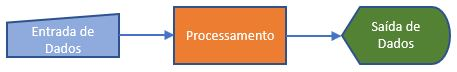
\includegraphics{images/03-01.jpg}
\caption{\label{fig:03-01}Etapas típicas de um programa}
\end{figure}

Programas mais sofisticados podem ter várias etapas distintas de entradas, utilizar dados de fontes diversas, podem ter o processamento subdividido em partes específicas, além de produzir várias saídas enviadas para destinos diferentes. As possibilidades, embora infinitas, são variações do tema \emph{entrada-processamento-saída}.

Os programas Python são executados pelo interpretador da linguagem que, \emph{naturalmente}, utiliza o console da plataforma, ou seja, o ambiente interativo e em modo texto oferecido pelos sistemas operacionais, mais conhecidos como \emph{prompt de comandos} no Microsoft Windows ou como \emph{terminais} nas distribuições Linux, Apple Mac OS e outros sistemas semelhantes. O console é composto por dois dispositivos: o teclado, considerado como a \emph{entrada-padrão}, e o monitor, tratado como \emph{saída-padrão} de todos esses sistemas operacionais.

Sendo assim, as operações de \emph{entrada} e de \emph{saída} realizadas no console dos sistemas são essenciais.

\hypertarget{e-s-saida}{%
\section{Saída Simples}\label{e-s-saida}}

A apresentação de resultados é uma etapa fundamental de qualquer programa, pois permite comunicar ao usuário informações sobre andamento do programa, bem como os resultados produzidos e, até mesmo, erros ou avisos sobre situações específicas encontradas durante sua execução.

A função \emph{built-in} \texttt{print()} tem como objetivo escrever os argumentos que recebe na \emph{saída-padrão}, ou seja, no console, produzindo texto legível pelo usuário como resultado. Sua sintaxe é simples:

\begin{quote}
\texttt{print(\ argumento*\ )}
\end{quote}

Tipicamente a função \texttt{print()} recebe um ou mais argumentos separados por vírgulas. Cada argumento pode ser uma \emph{string}, um número (inteiro, real ou complexo), um valor lógico ou uma variável, tal como segue:

\begin{Shaded}
\begin{Highlighting}[]
\BuiltInTok{print}\NormalTok{(}\StringTok{\textquotesingle{}Python, guia do programador\textquotesingle{}}\NormalTok{) }\CommentTok{\# str}
\BuiltInTok{print}\NormalTok{(}\DecValTok{2021}\NormalTok{) }\CommentTok{\# int}
\BuiltInTok{print}\NormalTok{(}\FloatTok{7.654321}\NormalTok{) }\CommentTok{\# float}
\BuiltInTok{print}\NormalTok{(}\VariableTok{True}\NormalTok{) }\CommentTok{\# bool}
\NormalTok{z }\OperatorTok{=} \FloatTok{1.2} \OperatorTok{{-}} \OtherTok{3.4j} \CommentTok{\# complexo}
\BuiltInTok{print}\NormalTok{(z) }\CommentTok{\# variável}
\end{Highlighting}
\end{Shaded}

\begin{verbatim}
>>> Python, guia do programador
>>> 2021
>>> 7.654321
>>> True
>>> (1.2-3.4j)
\end{verbatim}

Neste fragmento, cada uso de \texttt{print()} recebeu um único argumento, dos tipo \texttt{str}, \texttt{int}, \texttt{float}, \texttt{bool} e \texttt{complex}. O de tipo \texttt{str} foi \emph{transcrito} diretamente na saída-padrão, ou seja, no console, enquanto os demais foram convertidos para o tipo \texttt{str} e então exibidos.

Mas \texttt{print()} pode receber qualquer quantidade e combinação de tipos de argumentos, os quais devem ser separados por uma vírgula (\texttt{,}), o que oferece inúmeras possibilidades, como no próximo fragmento que combina o nome da variável na \emph{string} \texttt{\textquotesingle{}x\ =\textquotesingle{}} e o valor desta variável \texttt{x}:

\begin{Shaded}
\begin{Highlighting}[]
\NormalTok{x }\OperatorTok{=} \DecValTok{123456789}
\BuiltInTok{print}\NormalTok{(}\StringTok{\textquotesingle{}x =\textquotesingle{}}\NormalTok{, x)}
\end{Highlighting}
\end{Shaded}

\begin{verbatim}
>>> x = 123456789
\end{verbatim}

Aqui a função \texttt{print()} combinou um argumento do tipo \texttt{str} com outro do tipo \texttt{int}, convertendo cada um num texto, separado automaticamente por um espaço em branco, permitindo informar o usuário sobre o valor de uma variável específica do programa. O mesmo pode ser feito para mais variáveis, com textos complementares diversos.

\begin{Shaded}
\begin{Highlighting}[]
\NormalTok{x }\OperatorTok{=} \DecValTok{123456789}
\NormalTok{y }\OperatorTok{=} \DecValTok{9}
\BuiltInTok{print}\NormalTok{(}\StringTok{\textquotesingle{}x =\textquotesingle{}}\NormalTok{, x, }\StringTok{\textquotesingle{}e y =\textquotesingle{}}\NormalTok{, y)}
\end{Highlighting}
\end{Shaded}

\begin{verbatim}
>>> x = 123456789 e y = 9
\end{verbatim}

Além de valores literais, a função \texttt{print()} aceita expressões, de todos os tipos, como argumentos, ampliando ainda mais as maneiras de gerar saídas nos programas.

\begin{Shaded}
\begin{Highlighting}[]
\NormalTok{x }\OperatorTok{=} \DecValTok{123456789}
\NormalTok{y }\OperatorTok{=} \DecValTok{9}
\BuiltInTok{print}\NormalTok{(}\StringTok{\textquotesingle{}x * y =\textquotesingle{}}\NormalTok{, x }\OperatorTok{*}\NormalTok{ y)}
\end{Highlighting}
\end{Shaded}

\begin{verbatim}
>>> x * y = 1111111101
\end{verbatim}

Deve ser observado que \texttt{\textquotesingle{}x\ *\ y\ =\textquotesingle{}} é uma \emph{string} (um literal do tipo \texttt{str}), pois está delimitada por aspas-simples, enquanto \texttt{x\ *\ y} é uma expressão que envolve o produto das variáveis \texttt{x} e \texttt{y}, definidas no início do fragmento. Além disso, note que, no resultado produzido (\emph{impresso no console}), a função \texttt{print()} adicionou um espaço em branco entre os dois argumentos, tornando-os mais claros.

\hypertarget{e-s-saida-escap}{%
\subsection{Caracteres Especiais}\label{e-s-saida-escap}}

Nos literais de texto, isto é, nas \emph{strings}, é possível acrescentar caracteres especiais, em geral, caracteres \emph{não imprimíveis}, como a quebra-de-linha, que oferecem maior controle sobre as mensagens exibidas por um programa. A Tabela 3.1 lista os caracteres especiais do Python, conhecidos também como \emph{escape characters}.

Tabela 3.1: Caracteres especiais do Python

\begin{longtable}[]{@{}ll@{}}
\toprule
Código & Descrição \\
\midrule
\endhead
\texttt{\textbackslash{}\textquotesingle{}} & Aspas simples \\
\texttt{\textbackslash{}"} & Aspas duplas \\
\texttt{\textbackslash{}\textbackslash{}} & Barra invertida (\emph{backslash}) \\
\texttt{\textbackslash{}n} & Nova linha (\emph{new line}) \\
\texttt{\textbackslash{}r} & Retorno de carro (\emph{carriage return}) \\
\texttt{\textbackslash{}t} & Tabulação \\
\texttt{\textbackslash{}b} & Retrocesso (\emph{backspace}) \\
\texttt{\textbackslash{}o} & Prefixo para valor octal \\
\texttt{\textbackslash{}x} & Prefixo para valor hexadecimal \\
\bottomrule
\end{longtable}

Todos os caracteres especiais são, na verdade, sequências de dois caracteres, onde o primeiro é obrigatoriamente a barra invertida (\texttt{\textbackslash{}}). Assim, para que a própria barra invertida possa fazer parte de uma \emph{string}, ela deve ser indicada como a sequência de escape \texttt{\textbackslash{}\textbackslash{}}.

As aspas simples e duplas são os caracteres delimitadores das \emph{strings}, assim devem ser precedidas por uma barra invertida para que possam fazer parte da própria \emph{string}. O fragmento que segue mostra como incorporar as aspas e a barra invertida em \emph{strings} exibidas pela função \texttt{print()}.

\begin{Shaded}
\begin{Highlighting}[]
\NormalTok{texto\_1 }\OperatorTok{=} \StringTok{\textquotesingle{}Uso de aspas }\CharTok{\textbackslash{}\textquotesingle{}}\StringTok{simples}\CharTok{\textbackslash{}\textquotesingle{}}\StringTok{\textquotesingle{}}
\NormalTok{texto\_2 }\OperatorTok{=} \StringTok{"ou }\CharTok{\textbackslash{}"}\StringTok{duplas}\CharTok{\textbackslash{}"}\StringTok{ e da barra }\CharTok{\textbackslash{}\textbackslash{}}\StringTok{!"}
\BuiltInTok{print}\NormalTok{(texto\_1, texto\_2)}
\end{Highlighting}
\end{Shaded}

\begin{verbatim}
>>> Uso de aspas 'simples' ou "duplas" e da barra \!
\end{verbatim}

Também é possível incluir tabulações e quebras de linha numa \emph{string}, com o uso das sequências de escape \texttt{\textbackslash{}t} e \texttt{\textbackslash{}n} respectivamente. A tabulação introduz um espaçamento horizontal, cujo tamanho, de fato, depende do programa ou interface em uso, embora seja comum sua sua expansão para 4 ou 8 espaços. Observe o fragmento que segue, onde uma mesma frase é impressa quatro vezes, sem e com o uso de tabulação e quebra de linha.

\begin{Shaded}
\begin{Highlighting}[]
\BuiltInTok{print}\NormalTok{(}\StringTok{"Um texto simples"}\NormalTok{)}
\OperatorTok{\textgreater{}\textgreater{}\textgreater{}}\NormalTok{ Um texto simples}
\BuiltInTok{print}\NormalTok{(}\StringTok{"}\CharTok{\textbackslash{}t}\StringTok{Um texto simples"}\NormalTok{)}
\OperatorTok{\textgreater{}\textgreater{}\textgreater{}}\NormalTok{     Um texto simples}
\BuiltInTok{print}\NormalTok{(}\StringTok{"Um texto}\CharTok{\textbackslash{}n}\StringTok{simples"}\NormalTok{)}
\OperatorTok{\textgreater{}\textgreater{}\textgreater{}}\NormalTok{ Um texto}
\OperatorTok{\textgreater{}\textgreater{}\textgreater{}}\NormalTok{ simples}
\BuiltInTok{print}\NormalTok{(}\StringTok{"Um}\CharTok{\textbackslash{}n}\StringTok{texto}\CharTok{\textbackslash{}n\textbackslash{}t}\StringTok{simples"}\NormalTok{)}
\OperatorTok{\textgreater{}\textgreater{}\textgreater{}}\NormalTok{ Um}
\OperatorTok{\textgreater{}\textgreater{}\textgreater{}}\NormalTok{ texto}
\OperatorTok{\textgreater{}\textgreater{}\textgreater{}}\NormalTok{     simples}
\end{Highlighting}
\end{Shaded}

Na saída produzida por este fragmento, percebemos que a inclusão de um \texttt{\textbackslash{}t} no início da \emph{string} produz um espaçamento em sua apresentação. Já o caractere especial \texttt{\textbackslash{}n} gera uma quebra de linha, dividindo a exibição da \emph{string} em duas linhas. Os efeitos destes caracteres e as demais sequências de escape pode ser combinado para criação de mensagens, como se vê no último uso de \texttt{print()}.

\hypertarget{e-s-saida-opcao}{%
\subsection{Controle de Separação e Finalização}\label{e-s-saida-opcao}}

Como visto nos exemplos anteriores, a função \emph{built-in} \texttt{print()} adiciona, por padrão, um espaço em branco entre a impressão dos argumentos fornecidos, além disso, após imprimir o último argumento, finaliza a impressão com um caractere \texttt{\textbackslash{}n}, preparando uma nova linha para a próxima impressão. Então temos três situações distintas no uso de \texttt{print()}:

\begin{enumerate}
\def\labelenumi{\arabic{enumi}.}
\tightlist
\item
  Uso sem argumentos: impressão gera apenas uma quebra de linha.
\end{enumerate}

\begin{Shaded}
\begin{Highlighting}[]
\BuiltInTok{print}\NormalTok{() }\CommentTok{\# sem argumentos}
\end{Highlighting}
\end{Shaded}

\begin{enumerate}
\def\labelenumi{\arabic{enumi}.}
\setcounter{enumi}{1}
\tightlist
\item
  Uso com um único argumento: a impressão adiciona um espaço em branco \emph{entre} os argumentos e uma quebra de linha (\texttt{\textbackslash{}n}) para finalizar a saída.
\end{enumerate}

\begin{Shaded}
\begin{Highlighting}[]
\BuiltInTok{print}\NormalTok{(}\StringTok{"Argumento\_1"}\NormalTok{) }\CommentTok{\# um argumento}
\OperatorTok{\textgreater{}\textgreater{}\textgreater{}}\NormalTok{ Argumento\_1}
\end{Highlighting}
\end{Shaded}

\begin{enumerate}
\def\labelenumi{\arabic{enumi}.}
\setcounter{enumi}{2}
\tightlist
\item
  Uso com dois ou mais argumentos: a impressão adiciona um espaço em branco \emph{entre} todos argumentos e uma quebra de linha (\texttt{\textbackslash{}n}) para finalizar a saída.
\end{enumerate}

\begin{Shaded}
\begin{Highlighting}[]
\BuiltInTok{print}\NormalTok{(}\StringTok{"Argumento\_1"}\NormalTok{, }\StringTok{"Argumento\_2"}\NormalTok{) }\CommentTok{\# dois argumentos}
\OperatorTok{\textgreater{}\textgreater{}\textgreater{}}\NormalTok{ Argumento\_1 Argumento\_2}
\end{Highlighting}
\end{Shaded}

Neste exemplos, foram usados apenas argumentos do tipo \emph{string} para facilitar a compreensão, mas poderiam ser de qualquer tipo, ou ainda expressões. A Figura \ref{fig:03-01} ilustra a inserção do separador e do finalizador realizada pelo \texttt{print()}.

\begin{figure}
\centering
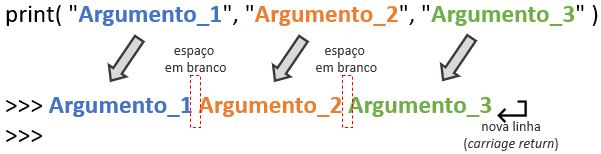
\includegraphics{images/03-02.jpg}
\caption{\label{fig:03-02}Inserção de separador e finalizador no \texttt{print()}}
\end{figure}

Além disso, a função \texttt{print()} permite que outro separador ou finalizador sejam utilizados, ampliando ainda mais suas possibilidades de uso. Isto é possível com a indicação explícita do parâmetro \texttt{sep} para escolha de um novo separador e do parâmetro \texttt{end} para escolha de um novo finalizador de impressão. Veja no fragmento que segue o uso da \emph{string} \texttt{-+-} como separador.

\begin{Shaded}
\begin{Highlighting}[]
\BuiltInTok{print}\NormalTok{(}\StringTok{"Argumento\_1"}\NormalTok{, }\StringTok{"Argumento\_2"}\NormalTok{, sep}\OperatorTok{=}\StringTok{\textquotesingle{}{-}+{-}\textquotesingle{}}\NormalTok{)}
\end{Highlighting}
\end{Shaded}

\begin{verbatim}
>>> Argumento_1-+-Argumento_2
\end{verbatim}

É fácil perceber que os argumentos passados para \texttt{print()} agora estão separados por \texttt{-+-}.

\begin{longtable}[]{@{}
  >{\centering\arraybackslash}p{(\columnwidth - 2\tabcolsep) * \real{0.12}}
  >{\raggedright\arraybackslash}p{(\columnwidth - 2\tabcolsep) * \real{0.88}}@{}}
\toprule
& \\
\midrule
\endhead

\includegraphics{images/application-green.png} & Para incluir o separador no início de uma impressão, ou em seu final, antes do finalizador, basta adicionar um argumento de tipo \emph{string} vazio, ou seja, \texttt{\textquotesingle{}\textquotesingle{}}, por exemplo:\texttt{print(\textquotesingle{}\textquotesingle{},\ \textquotesingle{}Argumento\ 1\textquotesingle{},\ \textquotesingle{}Argumento\ 2\textquotesingle{},\ \textquotesingle{}\textquotesingle{},\ sep=\textquotesingle{}\ \textbar{}\ \textquotesingle{})}que produz:\texttt{\textgreater{}\textgreater{}\textgreater{}\ \ \textbar{}\ Argumento1\ \textbar{}\ Argumento2\ \textbar{}} \\
\bottomrule
\end{longtable}

Segue outro fragmento que mostra o emprego do parâmetro \texttt{end} definido como ' separador \texttt{\textbar{}\textbar{}}.

\begin{Shaded}
\begin{Highlighting}[]
\BuiltInTok{print}\NormalTok{(}\StringTok{"Argumento\_1"}\NormalTok{, end}\OperatorTok{=}\StringTok{\textquotesingle{}||\textquotesingle{}}\NormalTok{)}
\BuiltInTok{print}\NormalTok{(}\StringTok{"Argumento\_2"}\NormalTok{)}
\end{Highlighting}
\end{Shaded}

\begin{verbatim}
>>> Argumento_1||
>>> Argumento_2
\end{verbatim}

Com isso, observamos que a sintaxe mais completa da função \emph{built-in} \texttt{print()} é, de fato:

\begin{quote}
\texttt{print(\ argumento*,\ sep=\textquotesingle{}\ \textquotesingle{},\ end=\textquotesingle{}\textbackslash{}n\textquotesingle{})}
\end{quote}

A função \texttt{print()}, embora simples, é muito flexível e seu uso indispensável.

\hypertarget{e-s-entra}{%
\section{Entrada}\label{e-s-entra}}

É comum que os programas sejam construídos para trabalhar seguindo as três etapas ilustradas na Figura \ref{fig:03-01}: efetuando uma \emph{entrada de dados}, seguida do \emph{processamento de dados}, que produz os resultados apresentados como sua \emph{saída de dados}. A entrada de dados é uma importante etapa que, em geral, dá início a esse processo.

A função \emph{built-in} \texttt{input()} tem como objetivo capturar dados fornecidos pelo usuário do programa na \emph{entrada-padrão}, usualmente o teclado, um dos dispositivos que fazem parte do console. Sua sintaxe é simples:

\begin{quote}
\texttt{variavel\ =\ input(\ prompt\ )}
\end{quote}

A função \texttt{input()} pode receber um argumento opcional do tipo \texttt{str}, ou seja, uma \emph{string} que serve como mensagem de orientação para o usuário, que deveria explica qual dado é esperado, ou seja, o tipo de dado a ser fornecido, a faixa de valores aceita ou outra característica esperada. Após a impressão da mensagem na \emph{saída-padrão}, aguarda que o usuário realize a digitação do dado, prosseguindo apenas quando é pressionada a tecla \texttt{ENTER}. Esta função então retorna o texto fornecido, usualmente armazenado em uma variável para uso futuro.

Isto significa que o uso de \texttt{input()} faz com que o programa pare sua execução, esperando pela digitação do usuário, prosseguindo apenas quando a \emph{entrada de dados} é finalizada com o acionamento de \texttt{ENTER}, armazenando o texto capturado na variável indicada pelo programador, o que é bastante conveniente.

\begin{Shaded}
\begin{Highlighting}[]
\NormalTok{nome }\OperatorTok{=} \BuiltInTok{input}\NormalTok{(}\StringTok{\textquotesingle{}Digite seu nome: \textquotesingle{}}\NormalTok{)}
\BuiltInTok{print}\NormalTok{(}\StringTok{\textquotesingle{}O nome digitado foi:\textquotesingle{}}\NormalTok{, nome)}
\end{Highlighting}
\end{Shaded}

\begin{verbatim}
>>> Digite seu nome: Peter
>>> O nome digitado foi: Peter
\end{verbatim}

Cada valor de entrada necessário à um programa deve ser lido por meio de uma chamada à função \texttt{input()}. Por exemplo;

\begin{Shaded}
\begin{Highlighting}[]
\NormalTok{nome }\OperatorTok{=} \BuiltInTok{input}\NormalTok{(}\StringTok{\textquotesingle{}Digite seu nome: \textquotesingle{}}\NormalTok{)}
\NormalTok{cidade }\OperatorTok{=} \BuiltInTok{input}\NormalTok{(}\StringTok{\textquotesingle{}Informe sua cidade: \textquotesingle{}}\NormalTok{)}
\BuiltInTok{print}\NormalTok{(}\StringTok{\textquotesingle{}Dados lidos:\textquotesingle{}}\NormalTok{, nome, }\StringTok{\textquotesingle{},\textquotesingle{}}\NormalTok{, cidade)}
\end{Highlighting}
\end{Shaded}

\begin{verbatim}
>>> Digite seu nome: Peter
>>> Informe sua cidade: Itatiba
>>> Dados lidos: Peter , Itatiba
\end{verbatim}

Embora o uso da função \texttt{input()} seja simples, é necessário destacar que todos os dados lidos são tratados como texto, ou seja, do tipo \texttt{str}. Considere o fragmento que segue.

\begin{Shaded}
\begin{Highlighting}[]
\NormalTok{a }\OperatorTok{=} \BuiltInTok{input}\NormalTok{(}\StringTok{\textquotesingle{}Digite um valor inteiro: \textquotesingle{}}\NormalTok{)}
\NormalTok{b }\OperatorTok{=} \BuiltInTok{input}\NormalTok{(}\StringTok{\textquotesingle{}Digite outro valor inteiro: \textquotesingle{}}\NormalTok{)}
\BuiltInTok{print}\NormalTok{(}\StringTok{\textquotesingle{}Valores lidos:\textquotesingle{}}\NormalTok{, a, }\StringTok{\textquotesingle{},\textquotesingle{}}\NormalTok{, b)}
\end{Highlighting}
\end{Shaded}

\begin{verbatim}
>>> Digite um valor inteiro: 12
>>> Digite outro valor inteiro: 34
>>> Valores lidos: 12 , 34
\end{verbatim}

Se o valor contido nas variáveis \texttt{a} e \texttt{b} for somado, teremos:

\begin{Shaded}
\begin{Highlighting}[]
\NormalTok{res }\OperatorTok{=}\NormalTok{ a }\OperatorTok{+}\NormalTok{ b}
\BuiltInTok{print}\NormalTok{(}\StringTok{\textquotesingle{}a + b =\textquotesingle{}}\NormalTok{, res)}
\end{Highlighting}
\end{Shaded}

\begin{verbatim}
>>> a + b = 1234
\end{verbatim}

O que parece ser um erro, na verdade está correto, pois a função \texttt{input()} trata todas as entradas fornecidas pelo usuário como texto, ou seja, valores do tipo \texttt{str}, que ao serem \emph{somados} são, de fato, \emph{concatenados}, ou seja, o texto de um operando é justaposto ao texto do outro operando. Podemos comprovar que a, b e res são do tipo \texttt{str} com:

\begin{Shaded}
\begin{Highlighting}[]
\BuiltInTok{print}\NormalTok{(}\StringTok{\textquotesingle{}type(a) =\textquotesingle{}}\NormalTok{, }\BuiltInTok{type}\NormalTok{(a), }\StringTok{\textquotesingle{}}\CharTok{\textbackslash{}n}\StringTok{type(b) =\textquotesingle{}}\NormalTok{, }\BuiltInTok{type}\NormalTok{(b), }\StringTok{\textquotesingle{}}\CharTok{\textbackslash{}n}\StringTok{type(res) =\textquotesingle{}}\NormalTok{, }\BuiltInTok{type}\NormalTok{(res))}
\end{Highlighting}
\end{Shaded}

\begin{verbatim}
>>> type(a) = <class 'str'> 
>>> type(b) = <class 'str'> 
>>> type(res) = <class 'str'>
\end{verbatim}

Para que possamos utilizar os dados fornecidos pelo usuário como valores numéricos, é necessário converter o texto lido no tipo de dados desejado. A conversão de texto para inteiro é feita com auxílio da função \emph{built-in} \texttt{int()}, que pode ser usada como segue:

\begin{Shaded}
\begin{Highlighting}[]
\NormalTok{a }\OperatorTok{=} \BuiltInTok{int}\NormalTok{(}\BuiltInTok{input}\NormalTok{(}\StringTok{\textquotesingle{}Digite um valor inteiro: \textquotesingle{}}\NormalTok{))}
\NormalTok{b }\OperatorTok{=} \BuiltInTok{int}\NormalTok{(}\BuiltInTok{input}\NormalTok{(}\StringTok{\textquotesingle{}Digite outro valor inteiro: \textquotesingle{}}\NormalTok{))}
\BuiltInTok{print}\NormalTok{(}\StringTok{\textquotesingle{}Valores lidos:\textquotesingle{}}\NormalTok{, a, }\StringTok{\textquotesingle{},\textquotesingle{}}\NormalTok{, b)}
\end{Highlighting}
\end{Shaded}

\begin{verbatim}
>>> Digite um valor inteiro: 12
>>> Digite outro valor inteiro: 34
>>> Valores lidos: 12 , 34
\end{verbatim}

Note que o resultado produzido por \texttt{input()}, que é o texto capturado como entrada do usuário, é passado como argumento da função \texttt{int()}, que realiza sua conversão para um valor inteiro. Agora é obtido o resultado esperado quando o valor contido nas variáveis \texttt{a} e \texttt{b} é somado:

\begin{Shaded}
\begin{Highlighting}[]
\NormalTok{res }\OperatorTok{=}\NormalTok{ a }\OperatorTok{+}\NormalTok{ b}
\BuiltInTok{print}\NormalTok{(}\StringTok{\textquotesingle{}a + b =\textquotesingle{}}\NormalTok{, res)}
\end{Highlighting}
\end{Shaded}

\begin{verbatim}
>>> a + b = 46
\end{verbatim}

A conversão de texto para valores reais, do tipo \texttt{float} é semelhante, como segue:

\begin{Shaded}
\begin{Highlighting}[]
\NormalTok{x }\OperatorTok{=} \BuiltInTok{int}\NormalTok{(}\BuiltInTok{input}\NormalTok{(}\StringTok{\textquotesingle{}Primeiro valor real: \textquotesingle{}}\NormalTok{))}
\NormalTok{y }\OperatorTok{=} \BuiltInTok{int}\NormalTok{(}\BuiltInTok{input}\NormalTok{(}\StringTok{\textquotesingle{}Segundo valor real: \textquotesingle{}}\NormalTok{))}
\NormalTok{z }\OperatorTok{=}\NormalTok{ x }\OperatorTok{+}\NormalTok{ y}
\BuiltInTok{print}\NormalTok{(}\StringTok{\textquotesingle{}Soma:\textquotesingle{}}\NormalTok{, z)}
\BuiltInTok{print}\NormalTok{(}\StringTok{\textquotesingle{}Produto:\textquotesingle{}}\NormalTok{, x }\OperatorTok{*}\NormalTok{ y)}
\end{Highlighting}
\end{Shaded}

Agora que sabemos como \emph{computar}, isto é, efetuar cálculos diversos, e também realizar as operações de \emph{entrada} e \emph{saída}, torna-se possível construir programas Python para resolver muitos tipos de problemas.

\begin{verbatim}
>>> Primeiro valor real: 3.45
>>> Segundo valor real: 8.76
>>> Soma: 12.21
>>> Produto: 30.222
\end{verbatim}

\begin{longtable}[]{@{}
  >{\centering\arraybackslash}p{(\columnwidth - 2\tabcolsep) * \real{0.12}}
  >{\raggedright\arraybackslash}p{(\columnwidth - 2\tabcolsep) * \real{0.88}}@{}}
\toprule
& \\
\midrule
\endhead

\includegraphics{images/application-yellow.png} & Atenção com o uso de \texttt{input()} quando são requeridos dados numéricos ou lógicos, pois isto requer transformar o texto lido no tipo desejado, usualmente com as funções \emph{built-int} \texttt{int()}, \texttt{float()} e \texttt{bool} que permitem as conversões para os respectivos tipos. \\
\bottomrule
\end{longtable}

\begin{longtable}[]{@{}
  >{\centering\arraybackslash}p{(\columnwidth - 2\tabcolsep) * \real{0.12}}
  >{\raggedright\arraybackslash}p{(\columnwidth - 2\tabcolsep) * \real{0.88}}@{}}
\toprule
& \\
\midrule
\endhead

\includegraphics{images/application-red.png} & Se o usuário fornece uma entrada inválida, isto é, que não pode ser convertida pelas funções \emph{built-int} \texttt{int()}, \texttt{float()} e \texttt{bool}, é lançada uma exceção \texttt{ValueError} indicando o problema. Além disso, caso esta exceção não seja tratada, o programa é abortado. \\
\bottomrule
\end{longtable}

\hypertarget{e-s-format}{%
\section{Saída Formatada}\label{e-s-format}}

Como veremos, em muitos programas surgirá a necessidade de apresentar os resultados de maneira mais organizada, eventualmente com uma aparência mais familiar para o usuário. Para isso, é necessária a aplicação de padrões de apresentação aos dados produzidos pelo programa, ou mais simplesmente, é necessário \emph{formatar} a saída.

Esta seção é dedicada a explorar capacidades um pouco mais avançadas do Python em relação a produção de saída de dados formatada. Exatamente por isso, sua leitura pode ser adiada até o momento em que sua necessidade se apresente, quando os exemplos dos próximos capítulos não forem suficientes para a compreensão das técnicas de formatação, ou quando um maior aprofundamento for desejado.

Existem algumas maneiras convenientes de produzir saída formatada no Python, obtido com:

\begin{itemize}
\tightlist
\item
  A função \emph{built-in} \texttt{format()};
\item
  A interpolação de \emph{strings} com \texttt{\%()}; e
\item
  As \emph{formatted literal strings}, ou simplesmente, as \emph{f-strings}.
\end{itemize}

\hypertarget{e-s-format-funcao}{%
\subsection{\texorpdfstring{Formatação com função \texttt{format()}}{Formatação com função format()}}\label{e-s-format-funcao}}

A função \emph{built-in} \texttt{format()} é destinada a converter um valor em sua representação \emph{formatada}, ou seja, aplica um padrão de apresentação, definido por uma \emph{string} que emprega uma sintaxe própria. Sua utilização permite controlar como valores numéricos e não numéricos são exibidos para o usuário. Esta função é indiretamente utilizada pela função de mesmo nome \href{https://docs.python.org/3/tutorial/inputoutput.html\#the-string-format-method}{\texttt{format()} da classe \texttt{str}}, com a sintaxe que segue:

\begin{quote}
\texttt{\textquotesingle{}padrao\_de\_formatacao\textquotesingle{}.format(\ *valor)}
\end{quote}

O padrão de formatação é uma \emph{string} na qual são inseridos \emph{marcadores de formatação} ou \emph{placeholders}, um para cada valor que se pretende formatar e exibir. Na função \texttt{format()}, aplicada ao \emph{padrão de formatação} por meio do operador \texttt{.} (denominado \emph{seletor}\footnote{No Python tudo é tratado como um objeto, até mesmo os literais numéricos e as \emph{strings}. Assim, o uso do operador \emph{seletor} possibilita o acesso aos métodos destes objetos, ou seja, às funções-membro que estão disponíveis em suas respectivas classes.}), devem ser dispostos os valores correspondentes aos marcadores de formatação. Seguem alguns exemplos para auxiliar na compreensão do uso da função \texttt{format()}.

Os \emph{marcadores de formatação} tem uma estrutura simples:

\begin{quote}
\texttt{\{\ {[}id{]}\ {[}:\ formato{]}\ \}}
\end{quote}

Todos os marcadores são delimitados por chaves obrigatórias, dentro das quais são dispostos um \texttt{id} e um \texttt{formato}, separados por dois-pontos quando o segundo elemento está presente. O \texttt{id} é um número inteiro opcional que pode ser utilizado para identificar um dos valores presentes em \texttt{format()}, o que permite sua reutilização, evitando sua repetição. Seu uso será visto mais à frente. O \texttt{formato} também é opcional e tem uma \href{https://docs.python.org/3/library/string.html\#formatspec}{sintaxe própria}, na qual são utilizados os especificadores relacionados na Tabela 3.2.

Tabela 3.2: Alguns especificadores de formatação do Python

\begin{longtable}[]{@{}cl@{}}
\toprule
Código & Descrição \\
\midrule
\endhead
\texttt{b} & Inteiro em formato binário (base 2) \\
\texttt{c} & Inteiro como caractere \\
\texttt{d},\texttt{n} & Inteiro decimal \\
\texttt{e},\texttt{E} & Real em notação científica \\
\texttt{f},\texttt{F} & Real com precisão fixa \\
\texttt{o} & Inteiro em formato octal (base 8) \\
\texttt{\%} & Porcentagem \\
\texttt{s} & String (cadeia de caracteres) \\
\texttt{x},\texttt{X} & Inteiro em formato hexadecimal (base 16) \\
\bottomrule
\end{longtable}

No fragmento que segue, o número inteiro contido na variável \texttt{x} é impresso sem aplicação de um padrão de formatação, mas como uso da função \texttt{format()}.

\begin{Shaded}
\begin{Highlighting}[]
\NormalTok{x }\OperatorTok{=} \DecValTok{15}
\BuiltInTok{print}\NormalTok{(}\StringTok{\textquotesingle{}}\SpecialCharTok{\{\}}\StringTok{\textquotesingle{}}\NormalTok{.}\BuiltInTok{format}\NormalTok{(x))}
\end{Highlighting}
\end{Shaded}

\begin{verbatim}
>>> 15
\end{verbatim}

Neste exemplo, o marcador vazio \texttt{\{\}} serve apenas para indicar onde o valor da variável \texttt{x} deve ser colocado na \emph{string de formatação}, funcionando como um \emph{marcador posicional}. Esta alternativa é bastante conveniente quando é necessário intercalar vários valores em uma mensagem, como no exemplo que segue.

\begin{Shaded}
\begin{Highlighting}[]
\NormalTok{x }\OperatorTok{=} \DecValTok{15}
\NormalTok{y }\OperatorTok{=} \DecValTok{19}
\BuiltInTok{print}\NormalTok{(}\StringTok{\textquotesingle{}Se x =\textquotesingle{}}\NormalTok{, x, }\StringTok{\textquotesingle{}e y =\textquotesingle{}}\NormalTok{, y, }\StringTok{\textquotesingle{}então x == y {-}{-}\textgreater{}\textquotesingle{}}\NormalTok{,}
\NormalTok{  x }\OperatorTok{==}\NormalTok{ y)}
\end{Highlighting}
\end{Shaded}

\begin{verbatim}
>>> Se x = 15 e y = 19 então x == y --> False
\end{verbatim}

\begin{Shaded}
\begin{Highlighting}[]
\BuiltInTok{print}\NormalTok{(}\StringTok{\textquotesingle{}Se x = }\SpecialCharTok{\{\}}\StringTok{ e y = }\SpecialCharTok{\{\}}\StringTok{, então x == y {-}{-}\textgreater{} }\SpecialCharTok{\{\}}\StringTok{\textquotesingle{}}
\NormalTok{  .}\BuiltInTok{format}\NormalTok{(x, y, x }\OperatorTok{==}\NormalTok{ y))}
\end{Highlighting}
\end{Shaded}

\begin{verbatim}
>>> Se x = 15 e y = 19, então x == y --> False
\end{verbatim}

No próximo fragmento, a função \texttt{print()} recebe uma \emph{string} de formatação que contém três marcadores: os dois primeiros, com a especificação do tipo do valor \texttt{\{:d\}}, recebem o conteúdo das variáveis \texttt{x} e \texttt{y}; e o último, um marcador posicional \texttt{\{\}}, recebe o resultado da expressão \texttt{x\ *\ y}.

\begin{Shaded}
\begin{Highlighting}[]
\NormalTok{x }\OperatorTok{=} \DecValTok{20}
\NormalTok{y }\OperatorTok{=} \DecValTok{6}
\BuiltInTok{print}\NormalTok{(}\StringTok{\textquotesingle{}}\SpecialCharTok{\{:d\}}\StringTok{ * }\SpecialCharTok{\{:d\}}\StringTok{ = }\SpecialCharTok{\{\}}\StringTok{\textquotesingle{}}\NormalTok{.}\BuiltInTok{format}\NormalTok{(x, y, x }\OperatorTok{*}\NormalTok{ y))}
\end{Highlighting}
\end{Shaded}

\begin{verbatim}
>>> 20 * 6 = 120
\end{verbatim}

Embora o efeito produzido aqui seja semelhante, o funcionamento destes marcadores é distinto. No marcador posicional, o valor correspondente é transformando numa \emph{string} inclusa na posição dada na \emph{string de formatação}, sendo indiferente o tipo do valor ali inserido. Já nos marcadores com especificadores é necessário que o valor correspondente seja de tipo compatível com o indicado, caso contrário será lançada a exceção \texttt{ValueError}.

Segue outro fragmento, onde outro número inteiro é exibido de maneiras diferentes. Observe que o padrão de formatação pode conter uma mensagem na qual se intercalam os marcadores de formatação desejados.

\begin{Shaded}
\begin{Highlighting}[]
\NormalTok{r }\OperatorTok{=} \DecValTok{12345}
\BuiltInTok{print}\NormalTok{(}\StringTok{\textquotesingle{}Valor não formatado }\SpecialCharTok{\{:d\}}\StringTok{ e com formato de 7 colunas }\SpecialCharTok{\{:7n\}}\StringTok{\textquotesingle{}}\NormalTok{.}\BuiltInTok{format}\NormalTok{(r, r))}
\end{Highlighting}
\end{Shaded}

\begin{verbatim}
>>> Valor não formatado 12345 e com formato de 7 colunas   12345
\end{verbatim}

Dois aspectos deve ser observados aqui: o uso direto de um especificador, tal como \texttt{d}, apenas apresenta o valor correspondente (o conteúdo da variável \texttt{r}), sem formatação; mas ao acrescentar o inteiro \texttt{7} como prefixo do especificador \texttt{n}, indica-se que o valor deverá ocupar sete colunas, ou seja, sua apresentação ocupará o espaço fixo de sete colunas (\emph{largura}). Este expediente pode ser utilizado com qualquer especificador para determinar a largura da apresentação.

Os especificadores para inteiros tem, então, a estrutura \texttt{{[}s{]}{[}w{]}d} ou \texttt{{[}s{]}{[}w{]}n} onde:

\begin{itemize}
\tightlist
\item
  \texttt{s}, opcional, indica como o sinal é mostrado: ausente ou \texttt{-}, apenas o sinal negativo é exibido; \texttt{+} exibe sinais positivos e negativos;
\item
  \texttt{w}, opcional, estabelece o número de colunas da largura da apresentação;
\item
  \texttt{d} ou \texttt{n} são os códigos dos especificadores para valores inteiros.
\end{itemize}

O fragmento que segue mostra o uso do indicador de sinal.

\begin{Shaded}
\begin{Highlighting}[]
\BuiltInTok{print}\NormalTok{(}\StringTok{\textquotesingle{}}\SpecialCharTok{\{:{-}8d\}}\StringTok{; }\SpecialCharTok{\{:{-}8n\}}\StringTok{\textquotesingle{}}\NormalTok{.}\BuiltInTok{format}\NormalTok{(}\DecValTok{123456}\NormalTok{, }\OperatorTok{{-}}\DecValTok{654321}\NormalTok{))}
\end{Highlighting}
\end{Shaded}

\begin{verbatim}
>>>   123456;  -654321
\end{verbatim}

\begin{Shaded}
\begin{Highlighting}[]
\BuiltInTok{print}\NormalTok{(}\StringTok{\textquotesingle{}}\SpecialCharTok{\{:+8d\}}\StringTok{; }\SpecialCharTok{\{:+8n\}}\StringTok{\textquotesingle{}}\NormalTok{.}\BuiltInTok{format}\NormalTok{(}\DecValTok{123456}\NormalTok{, }\OperatorTok{{-}}\DecValTok{654321}\NormalTok{))}
\end{Highlighting}
\end{Shaded}

\begin{verbatim}
>>>  +123456;  -654321
\end{verbatim}

\begin{longtable}[]{@{}
  >{\centering\arraybackslash}p{(\columnwidth - 2\tabcolsep) * \real{0.12}}
  >{\raggedright\arraybackslash}p{(\columnwidth - 2\tabcolsep) * \real{0.88}}@{}}
\toprule
& \\
\midrule
\endhead

\includegraphics{images/application-blue.png} & Quando a quantidade de caracteres necessárias para apresentar o valor dentro do padrão é menor do que largura indicada, espaços em branco são acrescentados, garantindo que o valor formatado ocupe a largura estabelecida. Nesta situação, os valores são alinhados à direita. Nada acontece quando a largura indicada é a mesma requerida pelo valor formatado. Mas, caso o valor requeira mais caracteres de apresentação do que a largura indicada, o padrão de formatação é desconsiderado e o valor é apresentado integralmente. \\
\bottomrule
\end{longtable}

Em algumas situações, um mesmo valor é utilizado mais de uma vez na saída produzida. Para evitar repetição do valor literal, variável ou expressão, podem ser empregados os \texttt{ids} nos marcadores para selecionar qual valor da lista contida em \texttt{format()} deve ser usado.

No fragmento que segue, a \emph{string} de formatação possui quatro marcadores, apenas com a indicação do \texttt{id}, onde o número \texttt{0} indica do primeiro valor da lista presente em \texttt{format()} (neste exempo a variável \texttt{x}), \texttt{1} indica o segundo (aqui a variável \texttt{y}) e assim sucessivamente.

\begin{Shaded}
\begin{Highlighting}[]
\NormalTok{x }\OperatorTok{=} \StringTok{\textquotesingle{}ra\textquotesingle{}}
\NormalTok{y }\OperatorTok{=} \StringTok{\textquotesingle{}qua\textquotesingle{}}
\BuiltInTok{print}\NormalTok{(}\StringTok{\textquotesingle{}A}\SpecialCharTok{\{0\}\{0\}\{1\}\{0\}}\StringTok{!\textquotesingle{}}\NormalTok{.}\BuiltInTok{format}\NormalTok{(x, y))}
\end{Highlighting}
\end{Shaded}

\begin{verbatim}
>>> Araraquara!
\end{verbatim}

Observe que o mesmo \texttt{id} pode ser indicado na \emph{string} de formatação, de maneira repetida e em qualquer ordem, evitando a repetição dos valores presentes em \texttt{format()}.

A formatação de números reais é bastante flexível, permitindo controlar não apenas a largura da apresentação, mas também o número de casas decimais exibidas e até mesmo a notação empregada.

No fragmento que segue o número real contido na variável \texttt{z} é impresso de quatro maneiras diferentes, genericamente, real sem formatação e com dois usos da notação de \emph{real com precisão fixa}, na qual se estabele um número fixo de casas decimais.

\begin{Shaded}
\begin{Highlighting}[]
\NormalTok{z }\OperatorTok{=} \FloatTok{123.456789}
\BuiltInTok{print}\NormalTok{(}\StringTok{\textquotesingle{}z = }\SpecialCharTok{\{0\}}\StringTok{ ou }\SpecialCharTok{\{0:f\}}\StringTok{ ou }\SpecialCharTok{\{0:8.2f\}}\StringTok{ ou }\SpecialCharTok{\{0:10.4f\}}\StringTok{!\textquotesingle{}}\NormalTok{.}\BuiltInTok{format}\NormalTok{(z))}
\end{Highlighting}
\end{Shaded}

\begin{verbatim}
>>> z = 123.456789 ou 123.456789 ou   123.46 ou   123.4568!
\end{verbatim}

Neste fragmento, todos os marcadores fazem uso do primeiro valor contido em \texttt{format()}. O primeiro marcador \texttt{\{0\}} exibe o valor como uma \emph{string}, sem verificar seu tipo. O segundo marcador, \texttt{\{0:f\}} verifica se o valor é um número real (de tipo \texttt{float}), mas sem aplicar qualquer formatação. Os demais marcadores aplicam a formatação de número \emph{real com precisão fixa}: \texttt{\{0:8.2f\}} indica apresentação com oito colunas no total, das quais uma para o separador decimal e duas casas decimais; enquanto \texttt{\{0:10.4f\}} requer apresentação com dez colunas no total, uma para o separador decimal e quatro casas decimais.

Os especificadores para reais tem, então, a estrutura \texttt{{[}s{]}{[}w{]}{[}.p{]}f} ou \texttt{{[}s{]}{[}w{]}{[}.p{]}e} onde:

\begin{itemize}
\tightlist
\item
  \texttt{s}, opcional, indica como o sinal é mostrado: ausente ou \texttt{-}, apenas o sinal negativo é exibido; \texttt{+} exibe sinais positivos e negativos;
\item
  \texttt{w}, opcional, estabelece o número de colunas da largura da apresentação;
\item
  \texttt{p}, opcional, complemento que indica o número de casas decimais apresentado;
\item
  \texttt{f} ou \texttt{e} são os códigos dos especificadores para valores reais, o primeiro para precisão fixa e o segundo para notação científica.
\end{itemize}

Quando \texttt{p} é indicado, aparece separado de \texttt{w} por um ponto, e determina o número de colunas da apresentação reservado para as casas decimais e o separador decimal.

O fragmento que segue exemplifica a formatação de uma variável real \texttt{z} com precisão fixa e com notação científica.

\begin{Shaded}
\begin{Highlighting}[]
\NormalTok{z }\OperatorTok{=} \FloatTok{123.456789}
\BuiltInTok{print}\NormalTok{(}\StringTok{\textquotesingle{}z = }\SpecialCharTok{\{0\}}\StringTok{ ou }\SpecialCharTok{\{0:.4f\}}\StringTok{ ou }\SpecialCharTok{\{0:+.4e\}}\StringTok{ ou }\SpecialCharTok{\{0:14.5E\}}\StringTok{!\textquotesingle{}}
\NormalTok{  .}\BuiltInTok{format}\NormalTok{(z))}
\end{Highlighting}
\end{Shaded}

\begin{verbatim}
>>> z = 123.456789 ou 123.4568 ou +1.2346e+02 ou    1.23457E+02!
\end{verbatim}

As \emph{strings} também podem ter sua exibição ser controlada com o especificador \texttt{s}, como mostra o fragmento que segue, onde barras verticais foram adicionadas para indicar os limites da \emph{string} impressa.

\begin{Shaded}
\begin{Highlighting}[]
\NormalTok{texto }\OperatorTok{=} \StringTok{\textquotesingle{}Peter Jandl Jr\textquotesingle{}}
\BuiltInTok{print}\NormalTok{(}\StringTok{\textquotesingle{}Nome: |}\SpecialCharTok{\{0\}}\StringTok{|}\CharTok{\textbackslash{}n}\StringTok{Nome: |}\SpecialCharTok{\{0:25s\}}\StringTok{|\textquotesingle{}}\NormalTok{.}\BuiltInTok{format}\NormalTok{(texto))}
\end{Highlighting}
\end{Shaded}

\begin{verbatim}
>>> Nome: |Peter Jandl Jr|
>>> Nome: |Peter Jandl Jr           |
\end{verbatim}

\begin{Shaded}
\begin{Highlighting}[]
\BuiltInTok{print}\NormalTok{(}\StringTok{\textquotesingle{}Nome: |}\SpecialCharTok{\{0:\textgreater{}25s\}}\StringTok{|}\CharTok{\textbackslash{}n}\StringTok{Nome: |}\SpecialCharTok{\{0:\^{}25s\}}\StringTok{|}\CharTok{\textbackslash{}n}\StringTok{Nome: |}\SpecialCharTok{\{0:\textless{}25s\}}\StringTok{|\textquotesingle{}}\NormalTok{.}\BuiltInTok{format}\NormalTok{(texto))}
\end{Highlighting}
\end{Shaded}

\begin{verbatim}
>>> Nome: |           Peter Jandl Jr|
>>> Nome: |     Peter Jandl Jr      |
>>> Nome: |Peter Jandl Jr           |
\end{verbatim}

O especificador \texttt{s} que tem a estrutura \texttt{{[}a{]}{[}w{]}s} onde:

\begin{itemize}
\tightlist
\item
  \texttt{a}, opcional, controla o alinhamento: \texttt{\textless{}} para esquerda, padrão para maioria dos objetos; \texttt{\textgreater{}} para direita, padrão para valores numéricos; \texttt{\^{}} para centralizado;
\item
  \texttt{w}, opcional, indica o número de colunas da largura da apresentação;
\item
  \texttt{s} é o código do especificador para \emph{string}.
\end{itemize}

A sintaxe dos especificadores é muito flexível, embora relativamente complexa, de maneira que sua \href{https://docs.python.org/3/library/string.html\#formatspec}{documentação} deve ser consultada sempre que necessário.

\hypertarget{e-s-format-inter} e uma série de valores. Observe o fragmento que segue, que produz a mesma saída formatada para uma variável real utilizando a função \texttt{format()} e a interpolação de \emph{string} equivalente.

\begin{Shaded}
\begin{Highlighting}[]
\NormalTok{n0 }\OperatorTok{=} \FloatTok{745.02}
\BuiltInTok{print}\NormalTok{(}\StringTok{\textquotesingle{}Valor = R$ }\SpecialCharTok{\{:7.2f\}}\StringTok{\textquotesingle{}}\NormalTok{.}\BuiltInTok{format}\NormalTok{(n0))}
\end{Highlighting}
\end{Shaded}

\begin{verbatim}
>>> Valor = R$  745.02
\end{verbatim}

\begin{Shaded}
\begin{Highlighting}[]
\BuiltInTok{print}\NormalTok{(}\StringTok{\textquotesingle{}Valor = R$ }\SpecialCharTok{\%7.2f}\StringTok{\textquotesingle{}} \OperatorTok{\%}\NormalTok{ (n0))}
\end{Highlighting}
\end{Shaded}

\begin{verbatim}
>>> Valor = R$  745.02
\end{verbatim}

Na interpolação de \emph{string}, cada marcador \texttt{\{\}} é substituído por um prefixo \texttt{\%} (\emph{placeholder}), usando a mesma sintaxe dos especificadores vistos seção \ref{e-s-format-funcao}; e o acionamento da função \texttt{format()} simplificado para \texttt{\%()}, onde deve ser relacionados um valor para cada \emph{placeholder}.

Este outro fragmento mostra a formatação de valores inteiros e reais, obtidos de variáveis e de expressões.

\begin{Shaded}
\begin{Highlighting}[]
\NormalTok{n1 }\OperatorTok{=} \DecValTok{190}
\NormalTok{n2 }\OperatorTok{=} \DecValTok{125}
\BuiltInTok{print}\NormalTok{(}\StringTok{\textquotesingle{}n1 = }\SpecialCharTok{\{:5d\}}\StringTok{, n2 = }\SpecialCharTok{\{:5d\}}\StringTok{, n1 / n2 = }\SpecialCharTok{\{:8.4f\}}\StringTok{\textquotesingle{}}\NormalTok{.}\BuiltInTok{format}\NormalTok{(n1, n2, n1 }\OperatorTok{/}\NormalTok{ n2))}
\end{Highlighting}
\end{Shaded}

\begin{verbatim}
>>> n1 =   190, n2 =   125, n1 / n2 =   1.5200
\end{verbatim}

\begin{Shaded}
\begin{Highlighting}[]
\BuiltInTok{print}\NormalTok{(}\StringTok{\textquotesingle{}n1 = }\SpecialCharTok{\%5d}\StringTok{, n2 = }\SpecialCharTok{\%5d}\StringTok{, n1 / n2 = }\SpecialCharTok{\%8.4f}\StringTok{\textquotesingle{}} \OperatorTok{\%}\NormalTok{ (n1, n2, n1 }\OperatorTok{/}\NormalTok{ n2))}
\end{Highlighting}
\end{Shaded}

\begin{verbatim}
>>> n1 =   190, n2 =   125, n1 / n2 =   1.5200
\end{verbatim}

A interpolação de \emph{string} é, em geral, um idioma mais compacto do que aquele requerido pela função \texttt{format()}, mas são, de fato equivalentes, portanto uma escolha pessoal de quem programa.

\hypertarget{e-s-format-fstring}{%
\subsection{\texorpdfstring{Formatação com \emph{f-string}}{Formatação com f-string}}\label{e-s-format-fstring}}

A versáo 3.6 do Python introduziu uma alternativa bastante interessante para formatação de saída denominada \href{https://docs.python.org/3/tutorial/inputoutput.html\#formatted-string-literals}{\emph{formatted string literals}} ou, mais simplesmente, \emph{f-string}. Além de ser uma notação mais compacta e simples, é menos inclinada a erros e também mais eficiente, devendo constituir a escolha preferencial para esta tarefa.

Uma \emph{f-string} deve ser iniciada com o prefixo \texttt{f} ou \texttt{F}. Nela podem ser inseridos um ou mais marcadores (\emph{placeholders}) para indicar onde valores, formatados ou não, devem ser inseridos, como no fragmento que segue:

\begin{Shaded}
\begin{Highlighting}[]
\NormalTok{f0 }\OperatorTok{=} \FloatTok{745.02}
\NormalTok{i1 }\OperatorTok{=} \DecValTok{2021}
\NormalTok{s3 }\OperatorTok{=} \StringTok{\textquotesingle{}Python\textquotesingle{}}
\BuiltInTok{print}\NormalTok{(}\SpecialStringTok{f\textquotesingle{}A linguagem }\SpecialCharTok{\{s3\}}\SpecialStringTok{, um valor inteiro }\SpecialCharTok{\{i1\}}\SpecialStringTok{ e outro real }\SpecialCharTok{\{f0\}}\SpecialStringTok{.\textquotesingle{}}\NormalTok{)}
\end{Highlighting}
\end{Shaded}

\begin{verbatim}
>>> A linguagem Python, um valor inteiro 2021 e outro real 745.02.
\end{verbatim}

O uso de uma \emph{f-string} torna direta a inserção de valores não formatados, que são diretamente indicados dentro de chaves \texttt{\{\}}.

A formatação dos valores requer a adição de um especificador para cada marcador, com a mesma sintaxe daqueles utilizados pela função \texttt{format()} (seção \ref{e-s-format-funcao}), como no exemplo que segue, que compara o uso de \texttt{format()} e de \emph{f-string}.

\begin{Shaded}
\begin{Highlighting}[]
\NormalTok{f0 }\OperatorTok{=} \FloatTok{745.02}
\BuiltInTok{print}\NormalTok{(}\StringTok{\textquotesingle{}Valor = R$ }\SpecialCharTok{\{:7.2f\}}\StringTok{\textquotesingle{}}\NormalTok{.}\BuiltInTok{format}\NormalTok{(f0))}
\end{Highlighting}
\end{Shaded}

\begin{verbatim}
>>> Valor = R$  745.02
\end{verbatim}

\begin{Shaded}
\begin{Highlighting}[]
\BuiltInTok{print}\NormalTok{(}\SpecialStringTok{f\textquotesingle{}Valor = R$ }\SpecialCharTok{\{n0:7.2f\}}\SpecialStringTok{\textquotesingle{}}\NormalTok{)}
\end{Highlighting}
\end{Shaded}

\begin{verbatim}
>>> Valor = R$  745.02
\end{verbatim}

Note que o valor a ser inserido (literal, variável ou expressão) é indicado diretamente dentro do marcador, que tem a estrutura \texttt{\{\textless{}valor\textgreater{}{[}:especificador{]}\}}, como no exemplo: \texttt{\{n0:7.2f\}}, onde \texttt{n0} é a variável, cujo valor é formatado, e \texttt{7.2f} é o especificador da formatação (número real, com 7 colunas de apresentação e duas casas decimais).

No próximo fragmento, é comparado o uso de \emph{interpolação de string} e de \emph{f-string} na exibição de duas variáveis inteiras e uma expressão de resultado real.

\begin{Shaded}
\begin{Highlighting}[]
\NormalTok{n1 }\OperatorTok{=} \DecValTok{190}
\NormalTok{n2 }\OperatorTok{=} \DecValTok{125}
\BuiltInTok{print}\NormalTok{(}\StringTok{\textquotesingle{}n1 = }\SpecialCharTok{\%5d}\StringTok{, n2 = }\SpecialCharTok{\%5d}\StringTok{, n1 / n2 = }\SpecialCharTok{\%8.4f}\StringTok{\textquotesingle{}} \OperatorTok{\%}\NormalTok{ (n1, n2, n1 }\OperatorTok{/}\NormalTok{ n2))}
\end{Highlighting}
\end{Shaded}

\begin{verbatim}
>>> n1 =   190, n2 =   125, n1 / n2 =   1.5200
\end{verbatim}

\begin{Shaded}
\begin{Highlighting}[]
\BuiltInTok{print}\NormalTok{(}\SpecialStringTok{f\textquotesingle{}n1 = }\SpecialCharTok{\{n1:5d\}}\SpecialStringTok{, n2 = }\SpecialCharTok{\{n2:5d\}}\SpecialStringTok{, n1 / n2 = }\SpecialCharTok{\{n1} \OperatorTok{/} \SpecialCharTok{n2:.4f\}}\SpecialStringTok{\textquotesingle{}}\NormalTok{)}
\end{Highlighting}
\end{Shaded}

\begin{verbatim}
>>> n1 =   190, n2 =   125, n1 / n2 = 1.5200
\end{verbatim}

As \emph{f-strings}, tanto por sua simplicidade, como flexibilidade e eficiência, devem ser usadas tanto quanto possível.

\hypertarget{seque}{%
\chapter{Sequenciação}\label{seque}}

A \emph{sequenciação} é a habilidade requerida para organizarmos uma sequência de instruções que permita resolver um problema específico. De muitas maneiras, sequenciar instruções é o mesmo que criar um \emph{algoritmo}\footnote{Dicio (Dicionário On-Line de Português): \url{https://www.dicio.com.br/algoritmo/}}, pois:

\begin{quote}
Na Matemática, representa um conjunto de regras para a resolução de um cálculo numérico, como, por exemplo, o algoritmo de Euclides encontra o máximo divisor comum de dois números inteiros. É também uma sequência de raciocínios ou operações que oferece a solução de certos problemas.
Na Informática, é um conjunto de regras que fornecem uma sequência de operações capazes de resolver um problema específico.
\end{quote}

Uma definição um pouco mais precisa do ponto de vista da Ciência da Computação seria:

\begin{quote}
Um algoritmo é uma sequência organizada e finita de instruções que permite a solução de um problema específico ou de uma classe de problemas.
\end{quote}

A habilidade da sequenciação trata, assim, de estabelecer uma sequência adequada de instruções para solução de um problema, ou seja, ela representa a lógica com a qual resolvemos um problema. A sequenciação determina como os dados de um problema serão processados, portanto combina todas as habilidades requeridas para a construção de programa de computador, que são a entrada e saída, a computação, a repetição, a decisão e a modularização.

\hypertarget{seque-progr}{%
\section{Programa Mínimo}\label{seque-progr}}

O comportamento \emph{natural} de um programa é ter suas instruções executadas uma a uma, da primeira até a última, na ordem em que se encontram. Isto é é o que se denomina \emph{fluxo sequencial}. As instruções, chamadas formalmente de diretivas (\emph{statements}), são separadas, no Python, por uma quebra de linha, de maneira que um programa é um texto, contendo uma, várias ou muitas instruções organizadas numa sequência.

Na verdade, o Python é bastante direto para a construção de seus programas, pois uma sequência simples de instruções constitui um programa, de modo que o menor programa possível, ou seja, o \emph{programa mínimo} seja aquele constituído de uma única instrução como no programa que segue, o clássico \href{https://www.thesoftwareguild.com/blog/the-history-of-hello-world/}{\emph{Hello World}}.

\begin{Shaded}
\begin{Highlighting}[]
\BuiltInTok{print}\NormalTok{(}\StringTok{\textquotesingle{}Hello, world!\textquotesingle{}}\NormalTok{)}
\end{Highlighting}
\end{Shaded}

\begin{verbatim}
>>> Hello, world!
\end{verbatim}

Esta simplicidade extrema torna o Python atraente tanto para aquele que está iniciando os estudos em programação, como para o especialista de outra área que pode se beneficiar da autonomia de criar seus próprios programas, assim como para os profissionais de Tecnologia da Informação que trabalham com desenvolvimento de software.

\hypertarget{repet}{%
\chapter{Repetição}\label{repet}}

Mais uma habilidade\ldots{}

\hypertarget{repet-while}{%
\section{Repetição Condicional}\label{repet-while}}

Dá-lhe \emph{while}!

\hypertarget{repet-for}{%
\section{Repetição Automática}\label{repet-for}}

Dá-lhe \emph{for}!

\hypertarget{decis}{%
\chapter{Decisão}\label{decis}}

\hypertarget{decis-if}{%
\section{Decisão Simples}\label{decis-if}}

Aqui tratamos do \emph{if}!

\hypertarget{decis-if-else}{%
\section{Decisão Completa}\label{decis-if-else}}

Aqui tratamos do \emph{if/else}!

\hypertarget{decis-if-elif-else}{%
\section{Decisões Encadeadas}\label{decis-if-elif-else}}

Aqui tratamos do \emph{if/elif/else}!

\hypertarget{modul}{%
\chapter{Modularização}\label{modul}}

\hypertarget{modul-main}{%
\section{Programa Principal}\label{modul-main}}

\hypertarget{modul-funcao}{%
\section{Funções}\label{modul-funcao}}

\hypertarget{modul-funcao-tipos}{%
\subsection{Tipos de funções}\label{modul-funcao-tipos}}

\hypertarget{modul-funcao-return}{%
\subsection{Retorno de Valor}\label{modul-funcao-return}}

\hypertarget{modul-funcao-param}{%
\subsection{Passagem de Parâmetros}\label{modul-funcao-param}}

\hypertarget{modul-funcao-default}{%
\subsection{\texorpdfstring{Parâmetros \emph{Default}}{Parâmetros Default}}\label{modul-funcao-default}}

\hypertarget{modul-funcao-var}{%
\subsection{Parâmetros Variáveis}\label{modul-funcao-var}}

\hypertarget{modul-import}{%
\section{Importação}\label{modul-import}}

\hypertarget{modul-packa}{%
\section{Criação de pacotes e módulos}\label{modul-packa}}

\hypertarget{appendix-apuxeandices}{%
\appendix}


\hypertarget{instalauxe7uxe3o-buxe1sica}{%
\chapter{Instalação básica}\label{instalauxe7uxe3o-buxe1sica}}

Blá blá blá blá blá blá blá blá blá blá blá blá blá blá blá blá blá blá blá blá blá blá blá blá blá blá blá blá blá blá blá blá blá blá blá blá blá blá blá blá blá blá blá blá blá blá blá blá blá blá blá blá blá blá blá blá blá blá blá blá blá blá blá blá blá blá blá blá blá blá blá blá blá blá blá blá blá blá blá blá blá blá blá blá blá blá blá blá blá blá blá blá blá blá blá blá blá blá blá blá blá blá blá blá blá blá blá blá blá.

Blá blá blá blá blá blá blá blá blá blá blá blá blá blá blá blá blá blá blá blá blá blá blá blá blá blá blá blá blá blá blá blá blá blá blá blá blá blá blá blá blá blá blá blá blá blá blá blá blá blá blá blá blá blá blá blá blá blá blá blá blá blá blá blá blá blá blá blá blá blá blá blá blá blá blá blá blá blá blá blá blá blá blá blá blá blá blá blá blá blá blá blá blá blá blá blá blá blá blá blá blá blá blá blá blá blá blá blá blá.

\hypertarget{instalauxe7uxe3o-do-anaconda}{%
\chapter{Instalação do Anaconda}\label{instalauxe7uxe3o-do-anaconda}}

Blá blá blá blá blá blá blá blá blá blá blá blá blá blá blá blá blá blá blá blá blá blá blá blá blá blá blá blá blá blá blá blá blá blá blá blá blá blá blá blá blá blá blá blá blá blá blá blá blá blá blá blá blá blá blá blá blá blá blá blá blá blá blá blá blá blá blá blá blá blá blá blá blá blá blá blá blá blá blá blá blá blá blá blá blá blá blá blá blá blá blá blá blá blá blá blá blá blá blá blá blá blá blá blá blá blá blá blá blá.

Blá blá blá blá blá blá blá blá blá blá blá blá blá blá blá blá blá blá blá blá blá blá blá blá blá blá blá blá blá blá blá blá blá blá blá blá blá blá blá blá blá blá blá blá blá blá blá blá blá blá blá blá blá blá blá blá blá blá blá blá blá blá blá blá blá blá blá blá blá blá blá blá blá blá blá blá blá blá blá blá blá blá blá blá blá blá blá blá blá blá blá blá blá blá blá blá blá blá blá blá blá blá blá blá blá blá blá blá blá.

  \bibliography{book.bib,packages.bib}

\end{document}
